\documentclass[a4paper,12pt]{article}

% --+ Packages +----------------------------------------------------------------
\usepackage[a4paper,top=2.5cm,bottom=3cm,left=3cm,right=3cm,marginparwidth=1.75cm]{geometry}
% \usepackage[document]{ragged2e} % Ragged left text.
\usepackage[english]{babel}
\usepackage{amsmath}    % Add \text to equations.
\usepackage{amssymb}    % \lesssim and \gtrsim.
\usepackage{booktabs}   % Beautiful tabular.
\usepackage{graphicx}   % Figures.
\usepackage{hvfloat}    % Include pdf file as page.
\usepackage{hyperref}   % Hyperlinks.
% \usepackage{incgraph}   % Include pdf file as page.
\usepackage{floatrow}   % Show figure source in a non-distracting manner.
\usepackage{listings}   % Code listings.
\usepackage{lmodern}    % Arbitrary font sizes.
\usepackage{mathtools}  % Subscript and superscript before symbol.
\usepackage{siunitx}    % SI units, used just for \micro.
\usepackage{subcaption} % Multiple figures together.
\usepackage{tabularx}   % \textwidth tabular.
\usepackage{textcomp, gensymb} % \degree.
\usepackage{textgreek}  % Greek letters in text mode.
\usepackage{titlesec}   % Custom sections.
\usepackage{wrapfig}    % Wrap text around figure.
\usepackage[font=small,labelfont=bf]{caption}

% --+ Setup 1 +-----------------------------------------------------------------
% Show only sections and subsections on TOC.
\setcounter{tocdepth}{2}

% Title formats.
\titleformat{\paragraph}{\normalfont\normalsize\bfseries}{\theparagraph}{1em}{}
\titleformat*{\subparagraph}{\normalfont\normalsize\bfseries}

% Code blocks setup (for pseudocode).
\lstset{basicstyle=\footnotesize,breaklines=true}

% gsim > gtrsim and lsim > lesssim.
\newcommand{\lsim}{\lesssim}
\newcommand{\gsim}{\gtrsim}

% custom overline from, https://tex.stackexchange.com/questions/22100/the-bar-and-overline-commands.
\makeatletter
\newsavebox\myboxA
\newsavebox\myboxB
\newlength\mylenA

\newcommand*\xoverline[2][0.75]{%
    \sbox{\myboxA}{$\m@th#2$}%
    \setbox\myboxB\null% Phantom box
    \ht\myboxB=\ht\myboxA%
    \dp\myboxB=\dp\myboxA%
    \wd\myboxB=#1\wd\myboxA% Scale phantom
    \sbox\myboxB{$\m@th\overline{\copy\myboxB}$}% Overlined phantom
    \setlength\mylenA{\the\wd\myboxA}% calc width diff
    \addtolength\mylenA{-\the\wd\myboxB}%
    \ifdim\wd\myboxB<\wd\myboxA%
       \rlap{\hskip 0.5\mylenA\usebox\myboxB}{\usebox\myboxA}%
    \else
        \hskip -0.5\mylenA\rlap{\usebox\myboxA}{\hskip 0.5\mylenA\usebox\myboxB}%
    \fi}
\makeatother

% Setup hyperlink color for PDF readers without link highlighting.
\hypersetup{colorlinks = true}
% \hypersetup{colorlinks = false} % NOTE. Remove color on hyperlinks for printing.

% --+ Document +----------------------------------------------------------------
\begin{document}
    % --+ Setup 2 +-------------------------------------------------------------
    \bibliographystyle{apalike}
    \pagenumbering{roman}

    % --+ First Pages +---------------------------------------------------------
    \graphicspath{{00first_pages/img}}
    % !TEX root = ../main.tex
% --+ Titlepage +---------------------------------------------------------------
\begin{titlepage}
\begin{center}
    \noindent
    \fontsize{18pt}{22pt}\selectfont Universidad T\'ecnica Federico Santa Mar\'ia \\
    \fontsize{16pt}{19pt}\selectfont Departamento de F\'isica \\
    \fontsize{16pt}{19pt}\selectfont Valpara\'iso, Chile \\
    \vspace{1.5cm}

    \includegraphics[width=4.41cm,height=3.34cm]{utfsm_shield.jpg}
    \vspace{1.5cm}

    \fontsize{20pt}{24pt}\selectfont ``Acceptance Study of the CLAS12 Detector Using the Forward Micromegas Tracker for Run Group E''
    \vfill
    \fontsize{16pt}{19pt}\selectfont Bruno Benkel
    \vfill
    \fontsize{16pt}{19pt}\selectfont Thesis Submitted for the Title of \\ Master in Science, Mention in Physics
    \vspace{1.5cm}

    \fontsize{14pt}{17pt}\selectfont Advisor: Hayk Hakobyan, PhD. \\
    \fontsize{14pt}{17pt}\selectfont Correferent Professor: Raffaella De Vita, PhD. \\
    \fontsize{14pt}{17pt}\selectfont Correferent Professor: Will Brooks, PhD.
    \vspace{2.5cm}

    \fontsize{14pt}{17pt}\selectfont June - 2023
\end{center}
\end{titlepage}

% --+ First pages +-------------------------------------------------------------
% !TEX root = ../main.tex
\setcounter{page}{2}
\
\vfill
\vfill
\begin{flushright}
    \noindent {\fontsize{16}{19}\selectfont \textbf{Dedication}}
\end{flushright}

\begin{flushright}
    \noindent
    Opa.
\end{flushright}
\vfill
       \pagebreak
% !TEX root = ../main.tex
\section*{Acknowledgements}
    % FMT Alignment team.
    \textbf{Raffaella De Vita}, Maxime Defurne, Veronique Ziegler.

    % RG-E Higher-ups.
    Hayk Hakobyan, Will Brooks, Taisiya Mineeva.

    % Eli.
    Eli Stensberg.

    % RG-F Team assistance.
    Mohammad Hattawy, Sebastian Kuhn.

    % Galil EPICS help.
    Nathan Baltzell, Mark Clift.

    % HIPO.
    Gagik Gavalian.

    % RG-E Target folks.
    Jairo Gonzales, Eduardo Valdivia, Sebastián Gálvez, Alonso Lepe, Nicole Benz.

    % RG-E Folks.
    Esteban Molina, Antonio Radic, Claudio San Martín, Matías Barria.

    % Family and stuff.
    Oma, Walter Benkel, Isabel Balbontin.
 \pagebreak
% !TEX root = ../main.tex
\section*{Abstract}
    \noindent \textbf{Abstract---}
        Particle accelerators and detectors are the main source of data for High Energy Physics.
        In this context, they are usually massive machines with a great number of moving parts, most of which require work in calibration and maintenance to run in optimal conditions.
        Special care must be put into the software dedicated to this calibration, in addition to event reconstruction.

        This thesis presents a calibration effort of this kind, done to the newest detector in the CLAS12 reconstruction chain --- the Micromegas Vertex Tracker.
        The results obtained in this regard are favourable.
        The calibration proved successful, doubling vertex resolution, and providing harsher criteria for selecting useful particle tracks.

        In addition, the thesis goes into detail about the improvements in reconstruction that come from this new detector, focusing on its acceptance, vertex resolution, and SIDIS variables.
        A full study is presented for the total acceptance in CLAS12, and the multiplicities of various types of particles are measured.

    \noindent \textbf{Keywords---}
        Particle detectors; Jefferson Laboratories; CLAS12; Micromegas Detectors.

    \vspace{1.0cm}

    \noindent \textbf{Resumen---}
        Los aceleradores y detectores de partículas son la principal fuente de datos para la Física de Altas Energías.
        En este contexto, estos suelen ser máquinas masivas con un gran número de partes móviles, la mayoría de las cuales requieren un trabajo de calibración y mantenimiento para funcionar en condiciones óptimas.
        Hay que tener especial cuidado en el \textit{software} dedicado a esta calibración, además del dedicado a la reconstrucción de eventos.

        Esta tesis presenta un trabajo en calibración de este tipo, realizado al detector más nuevo de la cadena de reconstrucción de CLAS12 --- el \textit{Micromegas Vertex Tracker}.
        Los resultados obtenidos son favorables.
        La calibración resultó exitosa, duplicando la resolución de vértice y proporcionando criterios más duros para la selección de \textit{tracks} de partículas útiles.

        Además, la tesis profundiza en las mejoras en reconstrucción que aporta este nuevo detector, centrándose en su \textit{acceptance}, la resolución de vértices y las variables de SIDIS.
        Se presenta un estudio completo de \textit{acceptance} total de CLAS12, y se miden las multiplicidades de varios tipos de partículas.

    \noindent \textbf{Palabras Clave---}
        Detectores de partículas; Jefferson Laboratories; CLAS12; Detectores Micromegas.
         \pagebreak
% !TEX root = ../main.tex
\section*{Glossary}
{\setlength{\parskip}{0cm}
    BAND:      Back Angle Neutron Detector \\
    BMT:       Barrel Micromegas Tracker \\
    CCDB:      Calibration and Conditions Database \\
    CD:        Central Detector \\
    CEBAF:     Continuous Electron Beam Accelerator Facility \\
    CLAS12:    CEBAF Large Acceptance Spectrometer for Operation at 12 GeV \\
    CND:       Central Neutron Detector \\
    CS-Studio: Control System Studio \\
    CTOF:      Central Time-of-Flight \\
    CVT:       Central Vertex Tracker \\
    DC:        Drift Chambers \\
    DIS:       Deep Inelastic Scattering \\
    DOCA:      Distance Of Closest Approach \\
    EB:        Event Builder \\
    EC:        Electromagnetic Calorimeter \\
    ECAL:      Electromagnetic Calorimeters \\
    ECIN:      EC-Inner \\
    ECOU:      EC-Outer \\
    EPICS:     Experimental Physics and Industrial Control System \\
    FD:        Forward Detector \\
    FMT:       Forward Micromegas Tracker \\
    FT:        Forward Tagger \\
    FTCal:     Forward Tagger Calorimeter \\
    FTOF:      Forward Time-of-Flight \\
    FTTrk:     Forward Tagger Gas Tracker \\
    FTHodo:    Forward Tagger Hodoscope \\
    GeV:       Giga electronVolt \\
    GUI:       Graphical User Interface \\
    HEP:       High Energy Physics \\
    HIPO:      High-Performance Input Output File Format \\
    HTCC:      High Threshold Cherenkov Counter \\
    IOC:       Input / Output Controller \\
    JLab:      Jefferson Laboratories \\
    linac:     Linear Particle Accelerator \\
    LTCC:      Low Threshold Cherenkov Counter \\
    MeV:       Mega electronVolt \\
    MM:        Micro-Mesh Gaseous Structure (Micromegas) \\
    mrad:      milliradian \\
    MVT:       Micromegas Vertex Tracker \\
    PID:       Particle Identification \\
    PCAL:      Pre-shower Calorimeter \\
    PDF:       Parton Distribution Function \\
    PMT:       PhotoMultiplier Tube \\
    pQCD:      perturbative Quantum Chromodynamics \\
    PV:        Process Variable \\
    QCD:       Quantum Chromodynamics \\
    RF:        Radio-Frequency \\
    RG-E:      Run Group E \\
    RG-F:      Run Group F \\
    RICH:      Ring Imaging Cherenkov Detector \\
    SVT:       Silicon Vertex Tracker \\
    SIDIS:     Semi-Inclusive Deep Inelastic Scattering \\
    T:         Tesla
}
         \pagebreak
\tableofcontents                         \pagebreak
\phantomsection \addcontentsline{toc}{section}{List of Figures}
\listoffigures                           \pagebreak


    \pagenumbering{arabic}
    % --+ Physics Motivation +--------------------------------------------------
    \graphicspath{{10physics_motivation/img}}
    % !TEX root = ../main.tex
\section{Physics Motivation} \label{sec::physicsmotivation}
    % --+ Introduction +--------------------------------------------------------
    % !TEX root = ../main.tex
% --+ Classical particle physics +----------------------------------------------
Since ancient times, humanity has pondered the composition of matter.
Philosophers from both East and West have often contemplated this question, and the modern view of this composition is based on the concept of the atom.
The notion of the atom, or indivisible particle, was proposed by Democritus in the 6th century B.C.
Despite its uncanny similarity to the modern concept of the atom, the model remained an abstract idea for more than two millennia.

In the grand scheme of things, it is only recently that we have been able to probe into the structure of matter and observe the atom.
In 1897, J.J. Thomson discovered "corpuscles," or electrons, using a cathode ray tube.
Based on this discovery, he proposed an atomic model consisting of a positively charged paste with lighter electrons floating inside.
Then, in 1909, Ernest Rutherford put this model to the test in what became the first scattering experiment in history.
By bombarding \textalpha particles onto a thin gold foil, he proved that most of the atom's mass was concentrated in a small, positively charged nucleus at its center.
He named the constituents of this nucleus protons.

Following that, Niels Bohr proposed the atomic planetary model in 1914.
His theory precisely fit the experimental data for Hydrogen but did not apply to heavier atoms.
This issue was resolved with the discovery of the neutron in 1932 by James Chadwick.
This discovery made the masses of atoms consistent with available experimental data, marking the end of the era of classical particle physics.

    % !TEX root = ../main.tex
% --+ The standard model +------------------------------------------------------
Then, in the 1950s and 1960s, a bewildering variety of particles were found in scattering experiments.
The theory born from this ``particle zoo'' gave rise to the Standard Model, which explains these particles as combinations of a small number of fundamental particles.
The model describes three of the four fundamental forces using force-mediating gauge bosons.
Additionally, it describes 24 particles, which are the constituents of matter.
Finally, it also includes one scalar boson, the Higgs boson, whose existence was proven in 2012 \cite{aad2012}.

Half of these 24 particles are elementary constituents of hadrons.
They were initially referred to as quarks by Murray Gell-Mann and George Zweig, and later as partons by Richard Feynman.
Quarks are point-like spin-1/2 particles with a fraction of an electron's electric charge, and they are distinguished by "flavors".
Both Gell-Mann and Zweig's constituent quark model and Feynman's parton model were later merged into the Quark-Parton model \cite{perkins2000}.

\begin{figure}[t!]
    \frame{\includegraphics[width=\textwidth]{02standard_model.pdf}}
    \caption[The standard model.]
    {Fundamental particles in the Standard Model.}
    \floatfoot{Source: \href{https://commons.wikimedia.org/wiki/Main_Page}{Wikimedia Commons}.}
    \label{fig::10.02::standard_model}
\end{figure}

    % --+ How to study particle physics and DIS +-----------------------------------
Deep Inelastic Scattering (DIS) is the process used to investigate the interior of hadrons using leptons.
The process is similar to Rutherford scattering and provided the first experimental evidence of quarks.
DIS can be employed to delve even deeper into the structure of matter by utilising increasingly higher energies, thanks to Werner Heisenberg's uncertainty principle.

High-energy probes lead to asymptotic freedom, which is the property where the interactions between particles, such as quarks, become increasingly weak at shorter distances.
This implies that inside hadrons, quarks mostly move as free, non-interacting particles.
This allows for reliable calculation of event cross-sections in particle physics.

    % !TEX root = ../main.tex
% --+ Quantum Chromodynamics +--------------------------------------------------
Another important feature is colour confinement, which is the property of colour-charged particles that prevents their isolation.
Colour charge is the Quantum Chromodynamics (QCD) equivalent of electric charge.
There are three colour charges and their corresponding anticharges.
Quarks possess a single colour charge, while gluons, the force-mediators of the strong force, have a bi-colour charge.
In a state of equilibrium, the strong force confines quarks to be in close proximity, forming quark-antiquark pairs or 3-quark triplets in such a way that the net colour charge is neutral.

QCD describes these properties and models the quark strong interaction.
Similar to the electromagnetic force, the strength of the interaction is determined by the strong coupling constant \textalpha.
However, unlike the electromagnetic force, this constant weakens as distances decrease.

    % --+ What is this experiment +-------------------------------------------------
At a larger distance scale, or smaller resolution, confinement is expected to become visible.
The \textalpha value increases to values close to 1, and the perturbative treatment of QCD is not viable.
There is limited knowledge about the non-perturbative behaviour of QCD, and therefore, it mostly relies on phenomenological models at present.
The aim of the RG-E experiment is to gather new data on the hadronic structure in Semi-Inclusive Deep Inelastic Scattering (SIDIS).
Through this experiment, we hope to gain further insight into quark propagation and hadron formation.


    % --+ Contents +------------------------------------------------------------
    % !TEX root = ../main.tex
\subsection{Deep Inelastic Scattering} \label{sec::dis}
% --+ Basic description +-------------------------------------------------------
    In its simplest description, Deep Inelastic Scattering (DIS) is the scattering of an electron off a quark inside a nucleon.
    Figure \ref{fig::dis_diagram} shows the Feynman diagram of DIS.
    The four-momentum of the nucleon is $P$, that of the quark is $p$, and the initial and final four-momenta of the electron are $k$ and $k'$, respectively.
    If $k'$ is measured, then the momentum transferred to the hadron system by the virtual photon is $q = k - k'$.
    $q$ is a spacelike vector, conventionally denoted as $q^2 = -Q^2$.

    \begin{figure}[h!]
        \centering\frame{
        \includegraphics[width=0.6\textwidth]{10physicsmotivation/img/10dis_diagram.pdf}}
        \caption[DIS in QCD.]{DIS in QCD. The diagram describes the stream of momentum in the scattering of a high energy electron off a quark. The quark's wave function is incorporated in the nucleon's wave function. Source: Own elaboration.}
        \label{fig::dis_diagram}
    \end{figure}

    If $Q^2$ is high enough, the quark is knocked out of the nucleon.
    Soft processes like gluon emission and quark-antiquark pair production then occur to neutralise the colour.
    This transforms the knocked-out quark into a jet of hadrons.
    This jet propagates in the direction of the electron's transferred momentum.

% --+ Approximating the cross section +-----------------------------------------
    To approximate the cross section of the electron-nucleon scattering, we'll work on the center of mass reference frame.
    Here, the electron and nucleon are propagating towards each other with enough energy to let us ignore the mass of the latter.
    Due to this, the nucleon has almost lightlike momentum along the collision axis.
    Its constituent quarks must therefore also have lightlike momenta, almost collinear to the nucleon's.
    Hence, to first order approximation, we can say of the quark's momentum is
    \begin{equation*}
        p = \xi P,
    \end{equation*}
    where $\xi$ is the longitudinal fraction of the quark's momentum, and as such $0 < \xi < 1$.

    In leading order approximation, we can also ignore the gluon emission and exchange during the collision.
    Then, the cross section of the electron-nucleon scattering is equal to that of the electron-quark's for a given $\xi$, multiplied by the probability that the nucleon contains a quark with $\xi$ longitudinal momentum fraction, integrated over $\xi$.

    This calculation has the problem that the probability that the nucleon contains a quark with a particular momentum can't be calculated in perturbative QCD.
    It depends on the soft processes that define the structure of the nucleon as a bound state of quarks and gluons.
    We must therefore consider this probability an unknown function to be measured in the experiment.

    This kind of probability functions are called Parton Distribution Functions (PDF).
    A PDF can be used for all kinds of quarks, antiquarks, and gluons, and are incorporated inside the nucleon's wave function.
    For each parton $f$, its PDF is defined as
    \begin{equation*}
        P_f = f_f(\xi)d\xi.
    \end{equation*}
    Therefore, the cross section of the inelastic scattering of the electron off the nucleon in leading order approximation is
    \begin{equation*}
        \sigma\left( e^-(k) p(P) \rightarrow e^-(k') X \right) =
                \int_0^1d\xi \sum_f f_f(\xi) \cdot
                \sigma\left( e^-(k) q_f(\xi P) \rightarrow e^-(k') + q_f(p') \right)
    \end{equation*}
    where $X$ indicates the final hadronic state.
    One should remember that this equation is not an exact QCD prediction, but is the first-term expansion of $\alpha_s$.
    This approximation is the parton model \cite{halzen1991}.

% --+ The parton model +--------------------------------------------------------
    \begin{figure}[b!] % NOTE. Figure out source.
        \centering\frame{
        \includegraphics[width=0.8\textwidth]{10physicsmotivation/img/10q2_dependence_u.png}}
        \caption[$Q^2$ dependence of $x$ PDF for the $u$ quark.]{$xf_f(x)$ parton distribution functions for the $u$ quark when $Q = 2$, $Q = 20$, and $Q = 200$ GeV.
        The plots show the parton evolution effect according to the Altarelli-Parisi equations.}
        \label{fig::q2dependenceu}
    \end{figure}

    In the parton model, the cross section is
    \begin{equation}
        \label{eq::parton_model_cross_section}
        \frac{d^2\sigma}{dxdy} \left( e^-p \rightarrow e^-X \right) =
                \left( \sum_f xf_f \left( x, Q^2 \right) Q_f^2 \right)
                \frac{2\pi\alpha s}{Q^4} \left( 1 + \left( 1 - y \right)^2 \right),
    \end{equation}
    where $s \equiv 2P\cdot k$, $Q_f$ is the charge of the parton $f$, and $x$ and $y$ are the Bjorken variables, defined as
    \begin{equation*}
        x \equiv \frac{Q^2}{2P\cdot q}, \hspace{36pt} y \equiv \frac{2 P\cdot q}{s}.
    \end{equation*}
    In the nucleon's rest frame, $y = q^0/k^0$, and thus it is the energy transferred to the hadron by the incoming electron.

    Due to gluon radiation, the PDFs in equation \eqref{eq::parton_model_cross_section} have a weak dependence on $Q^2$.
    This leads to Bjorken scaling violation \cite{halzen1991}.
    When the structure functions are known for certain values of $Q^2$, they can be evolved to other values using the Dokshitser-Gribox-Lipatov-Altarelli-Parisi (DGLAP) equations \cite{dokshitzer1991}.

    Figure \ref{fig::q2dependenceu} shows the predictions of the Altarelli-Parisi equations for the evolution of the PDFs dependence on $Q^2$.
    Partons with large $x$ tend to radiate and move to states with lower $x$.
    Parallel to this, the radiations produce new partons with low $x$ values.
    With an increase in $Q^2$, the parton distributions decrease for large $x$ values, while quickly increasing for low $x$.
    At low $Q^2$, the wavelength of the virtual photon is too large to probe the partons, thus probing the proton as a whole.
    The validity range for the QCD-extended parton model is not precisely known, but is assumed to be valid for $Q^2 > 1 \text{ GeV}^2$, corresponding to a spatial resolution of about $0.2$ fm.

% --+ Strong Coupling Constant +------------------------------------------------
    \subsubsection{Strong Coupling Constant $\alpha_s$}
        Measuring the experimental value of $\alpha_s$ is important for perturbative QCD calculations.
        To do this, one should determine the overall scale of renormalisation.
        This is usually selected to be the mass of the neutral Bose particle $Z^0$, which is $91.19$ GeV.
        Additionally, one should fix the scheme of renormalisation, which defines the coupling constant in a given scale.
        The experimental results for $\alpha_s$ can be seen on figure

        \begin{figure}[b!] % NOTE. Figure out source.
            \centering\frame{
            \includegraphics[width=0.8\textwidth]{10physicsmotivation/img/11strong_coupling_constant_q.png}}
            \caption[$\alpha_s$ dependence on $Q^2$.]{Experimentally measured $\alpha_s$ dependence on $Q$.
            The measured values are compared with theoretical predictions of renormalised evolution with initial $\alpha_s(m_z) = 0.117$ GeV.}
            \label{fig::alpha_q_dependence}
        \end{figure}

    % % !TEX root = ../main.tex
\subsection{Semi-Inclusive Deep Inelastic Scattering}
\label{10.20::semi_inclusive_deep_inelastic_scattering}
    The previous section focused solely on the detection of the scattered electron in the inclusive reaction.
    However, in the case where one of the produced hadrons is identified, the event is referred to as semi-inclusive.
    The identification of this hadron provides information about the flavor of the quark that was struck.
    In SIDIS, it is possible to measure this flavor dependence.
    The identified hadrons in SIDIS are known as current fragments, and it is important to separate them in the analysis from the fragments originating from the target.

    % !TEX root = ../main.tex
\subsubsection{SIDIS Cross Section}
\label{10.21::sidis_cross_section}
    In SIDIS, the fragmentation process corresponds to very low $Q^2$ and is not calculable in perturbative QCD (pQCD).
    It is parameterised by fragmentation functions $D_f^h(Q^2, z)$, which measure the probability that an $f$-flavoured quark fragments into an $h$-type hadron with a fraction $z$ of the virtual photon energy ($E_h = z\nu$).

    In the quark-parton model, the cross section for $eN \rightarrow ehX$ is assumed to be the differential cross section from Equation \eqref{eq::10.21::parton_model_cross_section} multiplied by the fragmentation probability
    \begin{equation}
        \label{eq::10.21::fragmentation_probability}
        \frac{d^3\sigma(eN \rightarrow ehX)}{dxdQ^2dz} =
            \frac{d^2\sigma(eN \rightarrow eX)}{dxdQ^2} \cdot
            \frac{\sum_f e^2_f q_f(x,Q^2) D^h_f(Q^2,z)}{\sum_f e^2_f q_f(x,Q^2)}.
    \end{equation}

    It is assumed that the quasi-free scattering process and the fragmentary process are independent in the cross section.

    The hadron multiplicity per DIS event, denoted as $M_h(Q^2, z)$, is given by:
    \begin{equation*}
        M_h(Q^2,z) \equiv \frac{1}{\sigma} \frac{d^3\sigma(eN \rightarrow ehX)}{dQ^2dz} = \frac{\int dx \sum_f e^2_f q_f(x,Q^2) D^h_f(Q^2,z)}{\int dx \sum_f e^2_f q_f(x,Q^2)},
    \end{equation*}
    where $\sigma$ is the differential inclusive DIS cross section $\frac{d^2\sigma(eN \rightarrow eX)}{dxdQ^2}$.


    % % !TEX root = ../main.tex
\subsection{Hadronisation in the Nuclear Medium}
% --+ Introduction +------------------------------------------------------------
    Hadronisation is the process in which quarks and gluons form hadrons.
    When in the nuclear medium, this process is influenced by quark energy loss through two mediums: Gluon radiation and multiple quark-nucleon scattering.
    Moreover, hadron-nucleon interactions also affect the process if the hadronisation happens inside the nucleus.

    In the process, the primary experimental observable is the multiplicity of hadrons produced on a dense nucleus as compared to a light one -- such as deuterium.
    In the absence of attenuation from interactions with the medium, these two quantities should be identical, such that the ratio between multiplicities would be unity.
    The ratio of hadron multiplicities -- known as attenuation ratio -- is defined as
    \begin{equation*}
        R^h_{\text{att}}(z,\nu) = \frac
                {\left( \frac{1}{\sigma} \frac{d^2\sigma(eN \rightarrow ehX)}{dzd\nu} \right)_A}
                {\left( \frac{1}{\sigma} \frac{d^2\sigma(eN \rightarrow ehX)}{dzd\nu} \right)_{\prescript{2}{}{H}}},
    \end{equation*}
    where the derivative with respect to $Q^2$ is substituted with one with respect to $\nu$.
    The $\nu$ and $z$ dependence of this ratio can be used to study the nature of the hadron formation mechanism.

    One type of observable that can be isolated is the characteristic times for the distinct stages of the hadronisation process.
    The existence of these stages is dictated by two of the most fundamental properties in QCD.
    First, confinement: a coloured quark can only propagate for a limited distance.
    Second, causality: the equilibrium colour field of a hadron cannot be formed instantaneously.

% --+ Absorption of the virtual photon +----------------------------------------
    \subsubsection{Virtual Photon Absorption}
        First, there is the absorption of a virtual photon by a quark on a presumably brief time, $\ll 1 \text{ fm}/\text{c}$, governed by the virtual photon wavelength.

% --+ Production time +---------------------------------------------------------
    \subsubsection{Production Time}
        Then, there must be a stage in which the coloured quark propagates as a quasi-free particle.
        During this second stage there is a gluon radiation with a differential spectrum given by pQCD as
        \begin{equation*}
            d\omega^{q \rightarrow qg} =
                    \frac{\alpha_s(k_\perp^2)}{4\pi}
                    \frac{8}{3}\left[ 1 + \left( 1 - \frac{k}{E} \right)^2 \right]
                    \frac{dk}{k} \frac{dk_\perp^2}{k_\perp^2},
        \end{equation*}
        where $E$ is the quark energy, $k$ is the 4-momentum of the gluon, and $k_\perp$ its transverse momentum.
        The time associated to this stage is commonly referred to as the \textit{production time} \cite{kopeliovich2004}, and is the length of time in which the quark is deconfined.
        Production time is a characteristic of the propagating quark, and should be independent of the final hadron formed.

        To a very good approximation, in deep inelastic kinematics and at $x > 0.1$, the struck quark absorbs all the energy of the virtual photon.
        Thus, the initial energy of the struck quark should be $\nu$.
        This quantity is much larger than the quark's mass (assuming an up or down quark), and thus we'll ignore it in the treatment of this theory.

        Conservation of energy then tells us that the final energy of the hadron produced should be no greater than $\nu$.
        Additionally, the gluon radiation leads to a loss of energy, meaning that the hadron's energy should be below $\nu$.
        We can estimate this energy loss from the string model \cite{artru1974}.
        Its main parameter is the string tension $\kappa \approx 1 \text{ GeV}/\text{fm}$.
        The growth of the string creates an energy loss governed by this $\kappa$.
        Therefore, we can estimate the rate of vacuum energy loss as
        \begin{equation*}
            \frac{dE}{dx}\Big|_\text{vacuum} \approx 1 \text{ GeV}/\text{fm}.
        \end{equation*}

        If $z_h = E_h/\nu$ is the fraction of the struck quark's energy retained by the hadron, then $\nu(1 - z_h)$ is the energy loss through gluon radiation.
        Thus, an estimate of the distance of gluon emission is
        \begin{equation*}
            l_p = \frac{\nu(1 - z_h)}{\kappa},
        \end{equation*}
        and thus production time $\tau_p$ is $l_p/c$ \cite{kopeliovich2004}.

        As an example, for a $10$ GeV pion with $z_h = 0.6$, $l_p = 4$ fm -- the production time is of the order of only a few fm for JLab energies.

% --+ Formation time +----------------------------------------------------------
    \subsubsection{Formation Time}
        In the final stage of the hadronisation process, the struck quark finds partner quarks to neutralise its colour, thus ending the gluon radiation.
        This stage is characterised by the evolution of the pre-hadron to an ordinary hadron, and is commonly name
        The formation time is the time required to form the colour field of a hadron.
        This time should depend on the hadron being formed.

        Formation time is not directly related to confinement, but rather is a measure of the time required to form the non-perturbative colour field of the hadron, starting from a small colour-singlet object.
        This field generation time has a well known analogue in Quantum Electrodynamics (QED).

        We can build a simple estimate for the formation time.
        To form an hadron of radius $R$ from a point-like, single-colour singlet, the speed at which the field can arise (in its rest frame) is bound by the speed of light
        \begin{equation*}
            \tau^\text{rest}_\text{formation} > \frac{R}{c},
        \end{equation*}
        which, Lorentz-boosted into the lab frame, is
        \begin{equation*}
            \tau^\text{lab}_\text{formation} > \frac{E}{m^*} \frac{R}{c},
        \end{equation*}
        where $m^*$ is the mass of the propagating colour-singlet object.
        In principle, $m^*$ ranges from the mass of two bare quarks to the fully formed hadron mass $m_h$.
        Then, a lower limit for the formation time is given by setting $m^* = m_h$.

        While this estimate is a classical calculation, a quantum mechanical analysis taking into account gluon wavelength arrives at the same result \cite{dokshitzer1991}.

        For a concrete example, for a $10$ GeV pion -- mass of $0.139$ GeV and radius of $0.7$ fm --, the formation time should be at least $50.4$ fm.
        Thus, in total, one can expect a pion production time of $3.3$ fm and formation time of at least $50.4$ fm in the lab frame at JLab energies.


    \pagebreak

    % --+ Experiment +----------------------------------------------------------
    \graphicspath{{11experiment/img}}
    % !TEX root = ../main.tex
\section{Experiment}
\label{11::experiment}
    The Thomas Jefferson National Accelerator Facility (TJNAF) is a High Energy Physics (HEP) laboratory located in Newport News, Virginia, USA.
    For simplicity and to follow convention, the laboratory will be called Jefferson Lab (JLab) hereafter.
    At the site, there is a recirculating linear electron accelerator named the Continuous Electron Beam Accelerator Facility (CEBAF).
    This accelerator is capable of delivering a 12 GeV electron beam to four experimental Halls simultaneously: Halls A, B, C, and D.

    Different physics topics are studied in each of these halls.
    This thesis aims to provide a preparatory study for the Run Group E (RG-E) experiment, which will take place in Hall B, where the CEBAF Large Acceptance Spectrometer for operation at 12 GeV (CLAS12) is located.

    The first section provides a brief description of CEBAF at JLab.
    The second section then provides detailed information about CLAS12, including its central detector, forward detector, and offline event reconstruction.
    The third and final section discusses the RG-E experiment to be performed.

    % !TEX root = ../main.tex
\subsection{CEBAF}
\label{ssec::cebaf}
    \begin{figure}[b!]
        \centering\frame{
        \includegraphics[width=\textwidth]{100cebaf_diagram.jpg}}
        \caption[CEBAF.]{Simplified representation of CEBAF.
        Source: \hyperlink{jlab.org/}{jlab.org}.}
        \label{fig::cebaf}
    \end{figure}

    CEBAF consists of a pair of 1.4-km-long antiparallel superconducting radio-frequency (RF) linear accelerators (linacs) constructed 8 meters below the surface.
    The two accelerators are connected by two 180-degree arcs, each with a radius of 80 meters \cite{leemann2001}.
    A schematic diagram illustrating the design of CEBAF is provided in Figure \ref{fig::cebaf}.

    The recirculating arcs are composed of five separate beamline sections, allowing the beam to traverse each linac up to five times.
    Within each linac, the energy gain of the beam ranges from 0.8 GeV to 1.2 GeV, resulting in a final beam energy of approximately 12 GeV.
    CEBAF is specifically designed for high-energy electron beam experiments aimed at studying the structure of mesons, nucleons, and nuclei \cite{rode2010}.

    % !TEX root = ../main.tex
\subsection{CLAS12}
\label{11.200::clas12}
    \begin{figure}[b!]
        \frame{\includegraphics[width=\textwidth]{200clas12_diagram.png}}
        \caption[CLAS12.]
        {The CLAS12 detector in the Hall B beamline.
        The electron beam enters from the right and impinges on the target located in the center of the solenoid magnet shown at the right (upstream) end of CLAS12.
        The FD consists of the High Threshold Cherenkov Counter (HTCC) (yellow), the torus magnet (grey), the Drift Chambers (DC) tracking system (light blue), and another set of Cherenkov counters (hidden), time-of-flight scintillation counters (brown), and Electromagnetic Calorimeters (ECs) (red).
        Between the HTCC and the torus, the Forward Tagger (FT) is installed.
        The Central Detector (CD) consists of the Silicon Vertex Tracker (SVT) (hidden), which is surrounded by a Barrel Micromesh Tracker (BMT) (hidden), the Central Time-of-Flight (FTOF) system, and the Central Neutron Detector (CND) (blue).
        At the upstream end, a Back Angle Neutron Detector (BAND) (red) is installed.}
        \floatfoot{Source: \href{https://jlab.org/physics/hall-b/clas12}{CLAS12 wiki}.}
        \label{fig::11.200::clas12_diagram}
    \end{figure}

    The main detector in Hall B is CLAS12, used to study electro-induced nuclear and hadronic reactions \cite{burkert2020}.
    The spectrometer provides efficient detection of charged and neutral particles over a large fraction of the full solid angle.

    CLAS12 is based on two superconducting magnets: a solenoid magnet and a 5 T torus magnet.
    The detector is divided into two parts: the Forward Detector (FD) and the Central Detector (CD).
    The FD, aided by the torus magnet, covers the forward polar range from $5\degree$ up to $35\degree$, while the CD, aided by the solenoid magnet, covers the polar angles from $35\degree$ to $125\degree$.
    Both detectors have full azimuthal coverage.

    Trajectory reconstruction is performed using Drift Chambers (DC) in the forward direction, achieving a momentum resolution of less than $1\%$.
    In the central detector, trajectory reconstruction is done using a vertex tracker, resulting in a momentum resolution of less than $3\%$.
    Particle identification relies on Cherenkov counters, time-of-flight scintillators, and electromagnetic calorimeters \cite{burkert2020}.
    Fast triggering and high data-acquisition rates enable operation at a luminosity of $10^{35} \text{ cm}^{-2}\text{ s}^{-1}$ \cite{burkert2020}.

    A diagram of CLAS12 showing the position of each detector component is provided in Figure \ref{fig::11.200::clas12_diagram}.

    % !TEX root = ../main.tex
\subsubsection{Forward Detector}
\label{sssec::forwarddetector}
    % The Forward Detector (FD) is an essential component of the CLAS12 spectrometer designed to detect particles scattered at small polar angles in the forward direction.
    % It consists of several subdetectors that play crucial roles in particle identification, tracking, and timing measurements.
    %
    % Based on its polar coverage, the FD can be divided into two: the Forward Tagger (FT) and the FD proper.
    % The former detects particles with a polar angle between $2.5\degree$ and $4.5\degree$.
    % The latter detects those with a polar angle between $5\degree$ and $35\degree$.
    % A detailed description of each subdetector systems is provided in the following paragraphs.
    %
    % The Forwards Micromegas Tracker (FMT) is part of the FD, but is not included in this list.
    % The detectors is explored in detail in Section \ref{ssec::forwardsmicromegastracker}.

    \input{11experiment/211htcc}
    \input{11experiment/212dc}
    \input{11experiment/213ltcc}
    \input{11experiment/214ftof}
    \input{11experiment/215rich}
    \input{11experiment/216ecal}
    \input{11experiment/217ft}

    % !TEX root = ../main.tex
\subsubsection{Central Detector}
\label{sssec::centraldetector}
    In the CLAS12 Central Detector (CD), particles scattered from the target within the polar angle range of $35\degree$ to $125\degree$ are detected.
    The CD consists of various detectors that provide particle identification and tracking capabilities.
    Charged particles are detected in the Central Vertex Tracker (CVT) and the Central Time-of-Flight (CTOF) detector.
    Neutron detection is provided by the Central Neutron Detector (CND), which is located radially outside of the CVT and the CTOF.
    All detectors have full coverage in the azimuthal angle.

    \input{11experiment/221cvt}
    \input{11experiment/222ctof}
    \input{11experiment/223cnd}
    \input{11experiment/224band}

    % !TEX root = ../main.tex
\subsubsection{Offline Reconstruction}
\label{sssec::offline_reconstruction}
% --+ CLARA +-------------------------------------------------------------------
    The CLAS12 reconstruction and analysis process is facilitated by a data-stream processing framework called CLARA.
    CLARA adopts a service-oriented architecture, allowing the construction of software applications using micro-services that are connected via data-stream pipes \cite{gyurgyan2016}.

    In this framework, each service plays a specific role.
    It receives input data, processes it according to its functionality, and produces output data.
    The input and output data are organised in tabular structures known as ``banks'', which are configured by the service developer to match the specific requirements of the service.

    The services within CLARA form a data-flow path, where the output of one service becomes the input for the next service in the sequence.
    This design enables a flexible and versatile data processing application, as each service can be individually improved or replaced without necessitating structural changes to the framework.

    To ensure consistency and modularity, the CLAS12 services are extensions of an abstract reconstruction engine.
    This engine provides common components such as initialisation and event processing methods, reducing the development complexity of individual micro-services and enforcing a uniform structure throughout the framework.

    By leveraging the CLARA framework, the CLAS12 experiment benefits from a modular and adaptable data processing pipeline, allowing for efficient reconstruction and analysis of the collected data.
    The service-oriented architecture and data-stream processing approach contribute to the flexibility, scalability, and maintainability of the CLAS12 software framework.

    \begin{figure}[b!]
        \centering\frame{
        \includegraphics[width=\textwidth]{230recon_chain.pdf}}
        \caption[CLAS12 Reconstruction Chain.]{Graphical representation of the CLAS12 interdependencies between services and banks.
        The I/O service reads events from the input file and distributes them to the reconstruction services chain for processing.
        Each service reads the relevant banks, applies the reconstruction algorithm, and provides output banks that are passed to the next service in the chain.
        The Event Builder (EB) service is executed as last in the chain; it collects the relevant banks from all CLAS12 subsystems services and produces event, particle, and detector response banks that are written to the output file.
        Source: Own elaboration.}
        \label{fig::recon_chain}
    \end{figure}

% --+ CLAS12 reconstruction +---------------------------------------------------
    The CLAS12 data reconstruction process involves data reader services that access decoded detector data stored in banks.
    Each entry in the bank represents a decoded detector hit and contains information such as sector, layer, component, order, and digitised data like signal charge, amplitude, time, or pedestal.

    During the decoding stage, similar bank structures are created for various quantities required for event reconstruction, including hits, clusters, and tracks.
    Reconstruction algorithms specific to each CLAS12 subsystem fill these banks.
    The data persistence service appends and writes these banks to a file for later analysis.

    The reconstruction algorithms are implemented as services that operate on input banks and produce output banks, which are then passed to subsequent algorithms in the reconstruction chain.
    The order in which the services are chained reflects the overall sequence of CLAS12 event reconstruction and the dependencies between subsystems.

    The first step is the reconstruction of charged particle tracks in the Central and Forward Detector tracking systems, based on the recorded hit positions in the respective detectors.
    This process is known as ``hit-based'' tracking.

    Simultaneously, hits recorded in other detectors are processed to reconstruct the energy and time of the associated particle interactions.
    The Event Builder (EB) service matches these reconstructed quantities with the tracks based on position and time information.
    Hits that are not matched to any track are retained as neutral particle candidates.
    The EB also determines the event ``start time'' and identifies the reconstructed particles.

    Once the event start time is determined, a second iteration of forward tracking, known as ``time-based'' tracking, can be performed.
    This iteration incorporates the drift times in the Drift Chambers, providing improved tracking precision \cite{ziegler2020}.

    An overview of the composition of reconstruction application services, depicting the dependencies between the services, can be found in Figure \ref{fig::recon_chain}.

    \input{11experiment/231tracking}
    \input{11experiment/232particle_identification}


    % !TEX root = ../main.tex
\subsection{RG-E Experiment}
\label{11.300::rge_experiment}
    The RG-E experiment, to be conducted in Hall B, focuses on measuring the hadronic multiplicity ratio between various nuclei and deuterium.
    To achieve this, a double-target system is being constructed.
    This system will enable a precise comparison between a deuterium target and heavy solid targets such as carbon, aluminium, copper, tin, lead, and others.
    The primary objective of the experiment is to enhance our understanding of hadronisation in the nuclear medium, colour transparency, and nuclear short-range correlations.

    During the data acquisition process, both the cryo-target (deuterium) and a solid target will be exposed to the electron beam simultaneously.
    To minimize differences in acceptance corrections between the targets, efforts are made to maintain a minimal distance between them.
    However, it is crucial to ensure that the targets can still be differentiated during the reconstruction process.
    The work behind this thesis contributes to the experiment by improving the offline reconstruction methods prior to the actual experiment, with the aim of reducing the distance between the targets.
    Further details on this topic can be found in Section \ref{12::fmt_alignment_and_reconstruction}.

    Simultaneously positioning both targets in the beam allows for the cancellation of time-dependent systematic effects, thereby increasing the precision of the final results.
    These effects can include drifting gains and inefficient detector channels when measuring ratio-like observables.
    Since the target system will be placed in a vacuum, the switching between solid targets needs to be done remotely.
    It is essential to perform the switching quickly to maximise the beam time available for the experiment.

    The double target system is designed to enable switching between up to five different solid targets.
    Previous experiments, such as EG2 conducted on the former CLAS, have demonstrated that the design of the double target system offers significant advantages in reducing systematic uncertainties \cite{hakobyan2008}.
    The principle of the target system involves installing the solid targets on a carbon fibre band that slides on torlon rails.
    The movement of the band is accomplished using a piezo-motor, chosen for its insensitivity to magnetic fields.
    Figure \ref{fig::11.300::double_target} illustrates the proposed design of the double target system.

    \begin{figure}[b!]
        \frame{\includegraphics[width=\textwidth]{300double_target.png}}
        \caption[Double-target system]
        {Double-target system CAD render.}
        \floatfoot{Source: Render by Alonso Lepe, from the Double Target group.}
        \label{fig::11.300::double_target}
    \end{figure}

    To ensure the proper functioning of the target, a series of tests have been conducted.
    These tests cover various aspects of the target's operation and performance.
    They include:

    \begin{itemize}
        \item
            Movement under vacuum and high magnetic field:
            The target system has been tested to ensure that it can operate smoothly and reliably under vacuum conditions and in the presence of high magnetic fields.
            This is important to verify that the target's movement and positioning are not affected by these conditions.

        \item
            Radiation hardness of selected materials:
            The materials used in the target system have been tested for their resistance to radiation.
            This is crucial because the target may be exposed to radiation during the experiment.
            By assessing the radiation hardness of the materials, it can be ensured that they will maintain their structural integrity and functionality throughout the experiment.

        \item
            Heat removal tests:
            The target system has undergone heat removal tests to ensure that it can effectively dissipate heat generated during operation.
            It is essential to keep the target temperature well below its melting point to prevent any damage or degradation.
            By conducting heat removal tests, the target's cooling capabilities have been evaluated to ensure optimal performance and longevity.
    \end{itemize}

    These tests collectively aim to validate the target's operational robustness and reliability under the specific conditions of the experiment, thereby ensuring accurate and consistent data collection.

    % !TEX root = ../main.tex
\subsubsection{Slow Control System}
\label{sssec::slowcontrolsystem}
% --+ What is slow control +----------------------------------------------------
    A modern experimental physics experiment usually involves many moving parts and complex components that require constant monitoring and calibration.
    Additionally, continuous data collection is necessary.
    This task is accomplished through the use of slow control systems.
    These systems typically integrate the entire detector and experiment into one complex interface, facilitating easy access and maintenance.

% --+ What is EPICS +-----------------------------------------------------------
    The standard framework used in the context of HEP for achieving this is the Experimental Physics and Industrial Control System (EPICS).
    EPICS was developed at the Los Alamos National Laboratory (ANL) to facilitate data acquisition and control for such experiments.
    This framework offers a distributed process control system that includes software communication, functional subsystems for data acquisition, supervisory control, closed-loop control, channel archiving, and alarm management \cite{dalesio1991}.

    Similar to many HEP experiments, the slow control system of CLAS12 is based on EPICS \cite{boyarinov2020}.

% --+ EPICS installation on raspi +---------------------------------------------
    To enable the integration of the RG-E target into the CLAS12 slow control system, the author developed an EPICS support module and Input/Output Controller (IOC).
    This module was not created from scratch since the motor developers had already developed a generic support module for Galil motors \cite{farnswort2009}.
    The existing system proved to be capable of supporting the movement of the RG-E target system, requiring only the removal of unnecessary features and the addition of experiment-specific database variables.

    The RG-E IOC, along with the complete set of EPICS support modules necessary to run it, can be found at

    \begin{center}
        \hyperlink{https://github.com/bleaktwig/rge-epics-support}{\texttt{https://github.com/bleaktwig/rge-epics-support}}.
    \end{center}

    The EPICS module includes Process Variables (PVs) that have been added to facilitate the control of the RG-E target system.
    Below is a list of these PVs along with a brief description of each.
    The user-defined records database, where these PVs can be viewed and edited, is located at

    \begin{center}
        \texttt{\$EPICS\_BASE/support/galil/3-6/db/galil\_userdef\_records.template}.
    \end{center}

    \input{11experiment/311process_variables}
    \input{11experiment/312cs_studio}
    \input{11experiment/313alarm_system}



    \pagebreak

    % --+ FMT Alignment +-------------------------------------------------------
    \graphicspath{{12fmt_alignment/img}}
    % !TEX root = ../main.tex
\section{FMT Alignment and Reconstruction}
\label{sec::fmt_alignment_and_reconstruction}
    In paper, the Forwards Micromegas Tracker (FMT) offers a 3 to 10-fold increase in resolution when compared to DC \cite{aune2009}.
    Achieving this improvement requires work on the alignment and calibration of the detector, as well as the reconstruction from its data.
    This chapter focuses on the work carried out in this endeavor, specifically addressing alignment and reconstruction.

    The first section provides a detailed description of Micromegas detectors in general and the FMT in particular.
    Subsequently, the second and third sections discuss the efforts made in alignment and reconstruction, respectively.
    Finally, the fourth and final section of the chapter elaborates on the resolution improvement resulting from this work.

    % !TEX root = ../main.tex
\subsection{Forwards MicroMegas Tracker}
\label{ssec::forwards_micromegas_tracker}
% --+ Micromegas +--------------------------------------------------------------
    \begin{figure}[b!]
        \centering\frame{
        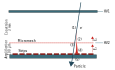
\includegraphics[width=\textwidth]{10mm_principle.pdf}}
        \caption[MM working principle.]{MicroMegas working principle.
        Source: Own elaboration.}
        \label{fig::mm_principle}
    \end{figure}

    A Micro-Mesh Gaseous Detector or MicroMegas (MM) is a gaseous particle detector that follows from the well-known wire chambers.
    These type of detectors are commonly used in experimental physics for the detection of ionising particles.
    The MM detector offers very precise temporal and spatial resolution, to the order of 100 nanoseconds and below 100 micrometers \cite{giomataris1996}.

    The detector works by amplifying the charges that have been created by ionisation in the gas volume.
    It's volume is separated into two parts by a metallic micro-mesh placed less than 150 micrometers of the readouts electrode or strip.

    For clarity, this process is exhibited in figure \ref{fig::mm_principle}.

    While passing through the detector, a particle will ionise the gas atoms by pulling up an electron, creating an electron ion pair (1).
    An electric field is applied to the gas ($\text{E}_1$), allowing the electron to drift toward the amplification electrode (2) and the ion towards the cathode.
    As the electron crosses the mesh (3), it enters an intense electric field ($\text{E}_2$), causing an avalanche effect (4).
    This creates a significant signal at the readout strip (5), which can be then stored for reconstruction \cite{giomataris1996}.

% --+ Micromegas in CLAS12 +----------------------------------------------------
    Inside the CLAS12 detector, a wide array of tracking detectors are used to figure out the positions and momenta of a particle at various points in its trajectory.
    The closer these detectors are to the source of a particle, the more precision is obtained about the position and momentum at the vertex of the interaction, i.e. the point where the particle was produced.
    In an attempt to maximise this precision, the MicroMegas Vertex Tracker (MVT) in CLAS12 is placed as close to the target as possible, as can be seen in figure \ref{fig::mvt}.

    \begin{figure}[b!]
        \centering\frame{
        \includegraphics[scale=0.5]{10mvt.png}}
        \caption[MVT detector.]{MVT detector.
        The red dot denotes the $z=0$ point in the beamline, the red line denotes an arbitrary track coming from that point, and the circumference in the Forward MicroMegas Tracker (FMT) denotes where that track produces a signal in an FMT layer.
        Source: \hyperlink{https://www.jlab.org/physics/hall-b/clas12}{CLAS12 wiki}.}
        \label{fig::mvt}
    \end{figure}

    Just as CLAS12 is divided into a central detector and a forward detector, the MVT is separated into two to maximise the angle coverage:
    The Barrel MicroMegas Tracker (BMT), a barrel tracker made of 18 cylindrical detectors arranged in 6 layers.
    This detector, in combination with the Silicon Vertex Tracker (SVT), covers the region from $35$ to $125\degree$ and greatly improves the polar angle resolution \cite{acker2020mvt}.

% --+ FMT +---------------------------------------------------------------------
    Then, the Forwards MicroMegas Tracker (FMT), which is made of six circular, flat detectors covering angles from $6$ to $29\degree$.
    In theory, it should improve the vertex resolution by a factor of $3$ to $10$ when compared to the Drift Chambers (DC) \cite{aune2009}.
    While the original design of the FMT included six layers, the current implemented detector has only three layers installed.
    This is due to technical difficulties and concerns regarding its Lorentz angle \cite{konczykowski2010}.

    Each of the three FMT layers has $1024$ readout strips, which follow a peculiar distribution, as can be seen in the image to the right of figure \ref{fig::fmt_geometry}.
    In addition, each layer's orientation differs by $60\degree$ to provide an accurate measurement in the xy-plane, as is shown in the image at the centre of the same figure \cite{acker2020mvt}.

    \begin{figure}[t]
        \centering\frame{
        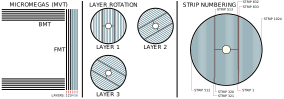
\includegraphics[width=\textwidth]{10fmt_geometry.pdf}}
        \caption[FMT detector geometry.]{FMT detector geometry. The first picture shows the distribution of the BMT and FMT layers, the second the different angle of each FMT layer, and the third the readout strip distribution of each FMT layer.
        Source: Own elaboration.}
        \label{fig::fmt_geometry}
    \end{figure}

\subsubsection{FMT Reconstruction}
    \begin{wrapfigure}{r}{0.50\textwidth}
        \centering\frame{
        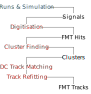
\includegraphics[width=\linewidth]{10fmt_recon.pdf}}
        \caption[FMT reconstruction summary]{FMT reconstruction summary.
        Data taking is coloured blue, data in black, and processes in red.
        Source: Own elaboration.}
        \label{fig::fmt_recon}
    \end{wrapfigure}

    After a signal is detected on a readout strip and the data is stored, information is obtained from it from offline reconstruction.
    Being a tracker, FMT's reconstruction works in a fairly similar manner to DC's.

    First, after a signal is detected in a strip it is digitised, processed, and turned into an \textbf{FMT Hit}.
    A group of FMT hits is processed via a \textbf{Cluster Finding} algorithm, where a \textbf{Cluster} is defined as a group of hits that supposedly come from the same particle track.
    A group of clusters from different layers go through a \textbf{DC Track Matching} algorithm, where they are matched to DC tracks from DC Reconstruction.
    A \textbf{Track Refitting} algorithm is applied for each DC track using the clusters' data, updating them to re-fitted tracks, named \textbf{FMT tracks}.
    This whole process is summarised in figure \ref{fig::fmt_recon}.

\clearpage

    % !TEX root = ../main.tex
\subsection{FMT Alignment}
\label{12.20::fmt_alignment}
% --+ Why is it needed +--------------------------------------------------------
    In an ideal scenario, the target and each detector would be installed precisely in their required positions.
    However, in the real world, there are inevitable misalignments in their placements.
    These misalignments must be accounted for and incorporated into the reconstruction process to ensure meaningful results.

    Within the CLAS collaboration, the Calibration and Commissioning group is responsible for the alignment and calibration of each detector.
    The shifts and rotations necessary for alignment are included in the Calibration and Conditions Database (CCDB), which is then utilised during reconstruction.

    The alignment work aimed to achieve three primary goals.
    Firstly, to provide FMT alignment tables to Run Group F (RG-F) for use in reconstruction.
    Secondly, to assess whether the resolution improvement obtained from the FMT justifies the additional material introduced into the CLAS12 detector.
    Lastly, to offer detailed information about these improvements, enabling Run Group E (RG-E) and other run groups to make informed decisions on whether to include the detector in their runs.

% --+ Definitions +-------------------------------------------------------------
    Alignment shifts can be performed in any of the three global axes: $z$, which is aligned with the beamline; $x$, which runs parallel to the ground; and $y$, which points upwards from the ground.
    Additionally, alignment rotations can be carried out around these axes.
    Specifically, for the purposes of this work, rotations around the $z$ axis are referred to as $\phi$ rotation (roll), while rotations around the $x$ and $y$ axes are termed pitch and yaw, respectively.

    To quantify misalignment, the DOCA between a reconstructed DC track and an FMT cluster is defined as a Residual.
    Due to the geometry of each layer (as depicted in Figure \ref{fig::12.10::fmt_geometry}), only the residuals in the local $y$ axis of a layer (perpendicular to the strips) can be measured.
    This implies that global $z$ and $\phi$ alignment can be performed independently for each layer.
    However, global $x$, global $y$, pitch, and yaw alignment must be carried out simultaneously for the entire detector.

% --+ How was it done +---------------------------------------------------------
    \begin{figure}[b!]
        \includegraphics[width=\textwidth]{20res_example.png}
        \caption[Example FMT residuals plot]
        {Example Forward Micromegas Tracker (FMT) residuals plot.}
        \floatfoot{Source: Own elaboration, using \href{https://github.com/JeffersonLab/clas12alignment}{CLAS12 alignment software}.}
        \label{fig::12.20::fmt_residuals_example}
    \end{figure}

    To minimise residuals, they are plotted for a specific shift or rotation in the relevant axes.
    An example of such a plot is illustrated in Figure \ref{fig::12.20::fmt_residuals_example}.
    Since the residuals are expected to follow a Gaussian distribution, a Gaussian fit is applied to them.

    For $z$ and $\phi$ alignment, the goodness of fit is heuristically evaluated by comparing the standard deviation ($\sigma$) of the Gaussian fits and selecting the shift with the smallest $\sigma$.
    For $x$, $y$, pitch, and yaw alignment, the goodness of fit is heuristically evaluated by choosing the fit with the mean closest to zero.
    It is important to consider a reasonable error margin when selecting the minima.

    Examples of the distributions of goodness of fit for $z$ and $xy$ alignment can be observed in Figure \ref{fig::12.20::fmt_residuals_fit_example}.

    \begin{figure}[t!]
        \includegraphics[width=\textwidth]{20resfit_example.png}
        \caption[Examples of residuals goodness of fit plots]
        {Examples of residuals goodness of fit plots.}
        \floatfoot{Source: Own elaboration, using \href{https://github.com/JeffersonLab/clas12alignment}{CLAS12 alignment software}.}
        \label{fig::12.20::fmt_residuals_fit_example}
    \end{figure}

    % !TEX root = ../main.tex
\subsubsection{Fiducial Cuts}
\label{sssec::fiducial_cuts}
    To reduce background, fiducial cuts are applied to the DC tracks and FMT clusters.
    This process is useful to increase data quality in order to obtain meaningful alignment results.

    For DC tracks, the cuts applied are:
    \begin{itemize}
        \item $\text{track}.z < \text{layer}.z$:
        Remove tracks with a vertex $z$ further downstream than the FMT layer before swimming.
        This is caused by reconstruction errors where the particle origin is outside of the target.
        % $9.84\%$ of tracks fail to meet this criterion in the sample data.
        \item $\mid\text{track}.z - \text{layer}.z\mid < 0.05 \text{cm}$:
        Remove tracks too far from the FMT layer after swimming.
        This was caused by bugs in the swimmer which will be mentioned in the next section.
        % $18.67\%$ tracks failed to meet this criterion.
        \item $5 \text{cm} < \sqrt{x^2 + y^2} < 25 \text{cm}$:
        Remove tracks outside of the layer's active region.
        % $35.22\%$ of the tracks were lost to this criterion.
        \item $\theta < ~66.42^{\circ}$:
        Remove tracks with a $\theta$ angle too high.
        When this happens, the same particle is affecting many strips, which causes the detector's data to not be as reliable as we want for alignment.
        % $7.22\%$ of tracks were lost to this criterion.
    \end{itemize}
    % From all these criteria, $70.95\%$ of the DC tracks were lost.
    % It is worth noting that after some reconstruction errors were fixed (as will be detailed in the following section), this percentage was reduced to $52.28\%$.

    For FMT clusters, the cuts applied are:
    \begin{itemize}
        \item $50 \text{ns} < \text{T}_{\text{min}} < 500 \text{ns}$:
        Cut clusters with an illogical $\text{T}_{\text{min}}$, which is the time of the first hit in the cluster.
        % $21.12\%$ of clusters fail to meet this criterion.
        \item $\text{size} > 1$ $\&\&$ $\text{E} > 100$:
        Cut small clusters with high energy, which are generally considered bad.
        % Only $7.36\%$ clusters are lost to this criterion.
        \item $\text{size} < 5$:
        Cut large clusters, which are not considered very useful.
        % Only $7.77\%$ are lost to this criterion.
    \end{itemize}
    % From all these criteria, $36.25\%$ of the FMT clusters were lost.

    % !TEX root = ../main.tex
\subsubsection{Residuals Improvements}
\label{12.22::residuals_improvements}
    To validate the proposed alignment algorithm, it was applied to the data from Run Group F (RG-F), specifically Run 11983.
    The improvement in residuals is readily apparent when comparing the before and after alignment results, as depicted in figure \ref{fig::12.22::fmt_residuals_comparison}.
    It is important to note the difference in scale between the top and bottom plots, which further highlights the significant improvement achieved through the alignment process.

    \begin{figure}[t!]
        \centering\frame{
        \includegraphics[width=\textwidth]{22res_comparison.png}}
        \caption[Residuals distribution improvement.]{Residuals distribution before (upper image) and after (lower image) alignment.
        Source: \hyperlink{github.com/JeffersonLab/clas12alignment}{CLAS12 alignment software}.}
        \label{fig::12.22::fmt_residuals_comparison}
    \end{figure}

    As depicted in the figure, the $z$ and $\phi$ alignment significantly reduces the background, resulting in a higher concentration of residuals around the mean of the distribution.
    Moreover, the $x$ and $y$ alignment effectively aligns the mean of the distribution closer to zero, improving the overall alignment.
    However, for the pitch and yaw alignment, meaningful results could not be obtained.
    This can be attributed to the limited data available from the three layers, combined with the small rotations around the $x$ and $y$ axes, making it challenging to achieve precise alignment.

    To determine the mean and standard deviation ($\sigma$) of the distribution, a Gaussian fit was applied. The parameters of the Gaussian fit are
     \begin{align*}
        \Big( \text{amp} \cdot \text{gaus}(\mu, \sigma) \Big) &+ \Big( p_0 + p_1\cdot x + p_2\cdot x^2 \Big) \\
        \text{gaussian} \hspace{0.8cm} &+ \hspace{1cm} \text{background}
    \end{align*}

    The results obtained are included in the CCDB at:

    \small\href{clasweb.jlab.org/cgi-bin/ccdb/versions?table=/geometry/fmt/alignment}{\texttt{clasweb.jlab.org/cgi-bin/ccdb/versions?table=/geometry/fmt/alignment}}

    Alignment was successfully performed for the data from Run Group M (RG-M), demonstrating that the alignment procedure is not specific to a particular run.
    This indicates the general applicability and effectiveness of the alignment procedure across different runs in the CLAS12 detector.

    The impact of this alignment procedure on the resolution of the entire CLAS12 detector will be further investigated and discussed in the concluding subsection of the section.


    The procedure described in this section is documented and shared publicly.
    It can be seen at

    \href{https://github.com/JeffersonLab/clas12alignment/tree/master/fmt}{\texttt{github.com/JeffersonLab/clas12alignment/tree/master/fmt}}

    % !TEX root = ../main.tex
\subsection{FMT Reconstruction Work}
\label{ssec::fmt_reconstruction_work}
% --+ Why is it needed +--------------------------------------------------------
    As the work on FMT alignment progressed, certain modifications were required in FMT reconstruction.
    These modifications primarily involved incorporating the alignment shifts determined during the alignment process into the reconstruction.
    Additionally, some fixes were made to address issues that were identified during the alignment work.
    These changes ensure that the reconstruction process takes into account the alignment information and addresses any related issues that were encountered.

% --+ What was done +-----------------------------------------------------------
    First, the loading of shifts from the CCDB was included in the standard geometry class of the FMT reconstruction package.
    Then, standard methods to include the shifts in any frame of reference change were implemented.
    Finally, the code was studied in detail, and the shifts were added in all instances where they were required since the package originally didn't consider their application.

    ``Crossmaking'' is the process of matching clusters in different layers to obtain an accurate 3D estimate of the position of a track \cite{ziegler2020}.
    This process was initially included in FMT reconstruction to facilitate the reconstruction for the six FMT layers.
    However, as mentioned before, only three FMT layers were installed for the RG-F run, and future runs may also use three layers due to concerns with the Lorentz angle when using six layers.
    To simplify the reconstruction process and make better use of the available number of layers, crossmaking was removed from the reconstruction.

    Outside of FMT reconstruction, some minor changes were also required in the DC reconstruction package since some of its components depend on the FMT layers' positions.
    Additionally, the swim package diagnostic was updated as it failed to properly reconstruct the positions of tracks near the FMT layers.

% --+ Juicy link +--------------------------------------------------------------
    A detailed list of the updates applied can be found in the following pull request to the \texttt{clas12-offline-software} repository:

    \href{github.com/JeffersonLab/clas12-offline-software/pull/726}{\texttt{github.com/JeffersonLab/clas12-offline-software/pull/726}}.

    % !TEX root = ../main.tex
\subsection{Validation and Results}
\label{ssec::validation_and_results}
% --+ Data used +---------------------------------------------------------------
    Just like the residuals validation, the results presented in this document are based on the application of this work to RG-F data.
    It is important to note that the RG-F target is approximately 55 centimetres long, which is much larger than the average CLAS12 target \cite{hattawy2019}.
    Specifically, the runs used for testing and validation are presented in Table \ref{tab::rgf_data}, and the run used to obtain the data displayed in this section was 011983.

    \begin{table}[h!]
        \centering
        \begin{tabular}{c|llll}
            \textbf{Run Number} & \textbf{Energy (MeV)} & \textbf{Current (nA)} & \textbf{Configuration} & \textbf{Target} \\
            \hline
            \textbf{011983}     & 10389.4 &  50 & Inbending & D2 \\
            \textbf{012016}     & 10389.4 & 250 & Inbending & D2 \\
            \textbf{012439}     &  2186.4 &  15 & Inbending & H2 \\
            \textbf{012461}     & 10196.6 &  20 & Inbending & D2
        \end{tabular}
        \caption{RG-F runs used for validation.}
        \label{tab::rgf_data}
    \end{table}

    % !TEX root = ../main.tex
\subsubsection{Cuts}
\label{sssec::cuts}
    \begin{figure}[b!]
        \centering\frame{
        \includegraphics[width=\textwidth]{40dc_vs_fmt.png}}
        \caption[DC vs FMT $z$ without geometric correction]{DC vs FMT vertex $z$ for electrons without any geometric correction. DC tracks are shown in green while FMT tracks are shown in blue. Note that the dark cyan colour comes from the overlap.
        Source: \texttt{fmtVertex.groovy} script in \hyperlink{github.com/JeffersonLab/clas12alignment}{CLAS12 alignment software}.}
        \label{fig::dc_vs_fmt_vz_011983}
    \end{figure}

    Some additional cuts are applied to the tracks to obtain the plots presented in this section.
    These cuts are used to remove very poor tracks that would not be suitable for analysis regardless.
    The applied cuts are as follows:
    \begin{itemize}
        \item
            \texttt{abs(chi2pid) < 5}:
            This cut removes tracks that do not provide sufficient certainty regarding the particle's PID.
        \item
            \texttt{vz < fmtZ}:
            This cut removes tracks located further downstream than the FMT.
        \item
            \texttt{chi2/ndf < 15}:
            This cut excludes tracks with excessively high uncertainty.
    \end{itemize}

    % !TEX root = ../main.tex
\subsubsection{Geometry Effect}
\label{sssec::geometry_effect}
    To evaluate the enhancement in vertex resolution, we will compare the vertex positions of tracks that underwent only DC reconstruction with those that underwent both DC and FMT reconstruction.
    For convenience, we will refer to the former as DC tracks and the latter as FMT tracks.
    Considering that the $z$ axis is aligned with the beamline, Figure \ref{fig::dc_vs_fmt_vz_011983} illustrates the $z$ positions of the vertex for DC tracks versus FMT tracks.

    To comprehend the plot in Figure \ref{fig::dc_vs_fmt_vz_011983}, it is valuable to examine the RG-F target.
    The target consists of a large gas-filled chamber with a varying composition across different runs.
    The distance between the chamber windows measures $553.32$ millimetres.
    Furthermore, it was observed that the upstream window of the target is positioned approximately $24$ millimetres away from the beam window.
    All windows are constructed from aluminium and have a thickness of $15$ micrometers.
    A detailed depiction of the target can be found in Addendum 1.

    Based on Figure \ref{fig::dc_vs_fmt_vz_011983}, it is evident that the FMT detector solely detects the upstream windows, completely overlooking the downstream one.
    This issue stems from a geometric constraint: the downstream window falls outside the active detection area of the FMT.
    This effect is clearly illustrated in Figure \ref{fig::vz_vs_theta}, where the $\theta$ angle is plotted against the vertex $z$ coordinate.
    The two red lines in the plots represent the FMT's active area, and it is apparent that the downstream window lies outside this region, thereby explaining its absence.

    \begin{figure}[t!]
        \centering\frame{
        \includegraphics[scale=0.24]{42theta_dc_vs_fmt.png}}
        \caption[$z$ vs $\theta$ for DC and FMT.]{$z$ vs $\theta$ for DC and FMT for electrons without any geometry correction. FMT's active area are shown in red lines.
        Source: \texttt{fmtVertex.groovy} script in \hyperlink{github.com/JeffersonLab/clas12alignment}{CLAS12 alignment software}.}
        \label{fig::vz_vs_theta}
    \end{figure}

    To account for this geometric effect, we apply an additional cut based on the plotted curves.
    The curves are given by
    \begin{equation} \label{eq::fmt_geometry_cut}
        c_1 = 57.29 \cdot \arctan\left(\frac{r_\text{inner}}{z_0 - z}\right), \hspace{0.5cm}
        c_2 = 57.29 \cdot \arctan\left(\frac{r_\text{outer}}{z_0 - z}\right),
    \end{equation}
    where $r_\text{inner}$ is the radius of the hole at the center of FMT, $r_\text{outer}$ is the radius of the outer circumference of FMT, and $z_0$ is the $z$ position of the first FMT layer plus the drift distance.
    All these parameters are read from the CCDB.

    To compensate for this geometric effect, we introduce an additional cut based on the plotted curves.
    The curves can be described by the following equations
    \begin{equation} \label{eq::fmt_geometry_cut}
        c_1(z) = 57.29 \cdot \arctan\left(\frac{r_\text{inner}}{z_0 - z}\right),
        \hspace{0.5cm}
        c_2(z) = 57.29 \cdot \arctan\left(\frac{r_\text{outer}}{z_0 - z}\right).
    \end{equation}

    Here, $r_\text{inner}$ represents the radius of the hole at the center of the FMT, $r_\text{outer}$ denotes the radius of the outer circumference of the FMT, and $z_0$ corresponds to the $z$ position of the first FMT layer plus the drift distance.
    All these parameters are obtained from the CCDB.

    % !TEX root = ../main.tex
\subsubsection{Vertex Resolution Improvement}
\label{12.43::vertex_resolution_improvement}
    Furthermore, an additional cut has been introduced.
    As of the FMT alignment work, beam alignment for RG-F data had not been carried out, resulting in a decrease in vertex resolution.
    To mitigate the impact of this alignment issue on reconstruction accuracy, we have implemented a cut to utilise only one sector of the detector.

    \begin{figure}[b!]
        \centering\frame{
        \includegraphics[scale=0.24]{40dc_vs_fmt_sector1.png}}
        \caption[DC vs FMT $z$ with geometry correction]{DC vs FMT vertex $z$ for electrons with a geometric correction. DC tracks are shown in green while FMT tracks are shown in blue. Data from only one CLAS12 sector was used to obtain this plot.
        Source: \texttt{fmtVertex.groovy} script in \hyperlink{github.com/JeffersonLab/clas12alignment}{CLAS12 alignment software}.}
        \label{fig::12.43::dc_vs_fmt_vz_11983_corrected}
    \end{figure}

    The resolution plot, comparing DC and FMT tracks after applying all the previously mentioned cuts, is depicted in Figure \ref{fig::12.43::dc_vs_fmt_vz_11983_corrected}.
    To evaluate the resolution for both DC and FMT tracks, we utilise a fit consisting of two Gaussian curves combined with a quadratic curve to account for the background.
    The fit is defined as follows
    \begin{equation*}
        \text{amp}_1 \cdot \text{gaus}(z, z_\text{max}, \sigma) + \text{amp}_2 \cdot \text{gaus}(z, z_\text{max} - 2.4, \sigma) + p_1 + p_2\cdot z + p_3\cdot z^2,
    \end{equation*}
    where
    \begin{itemize}
        \item
            $\text{amp}1$ represents the amplitude of the largest peak, and $z\text{max}$ corresponds to its $z$ position,
        \item
            $\text{amp}_2$ signifies the amplitude of the leftward peak, which has been measured to be at a position of $2.4$ centimetres, and
        \item
            the remaining parameters, $p_1$, $p_2$, and $p_3$, are obtained through the fitting process.
    \end{itemize}

% --+ Resolution for electrons +------------------------------------------------
    For electrons in run 011983 (low luminosity, 50 nA), the analysis yields a DC resolution of $\sigma_\text{DC} = 0.875$ cm and an FMT resolution of $\sigma_\text{FMT} = 0.387$ cm.
    This indicates a doubling of the resolution achieved with the inclusion of the FMT detector.

    Similarly, for electrons in run 012016 (production luminosity, $250$ nA), the analysis shows a DC resolution of $\sigma_\text{DC} = 1.009$ cm and an FMT resolution of $\sigma_\text{FMT} = 0.596$ cm.

    % !TEX root = ../main.tex
\subsubsection{Conclusions}
\label{12.44::conclusions}

    \begin{figure}[b]
        \frame{\includegraphics[width=\textwidth]{44fmt_efficiency.png}}
        \caption[FMT layers efficiency]
        {Efficiency of each FMT layer.}
        \floatfoot{Source: Own elaboration, using the \texttt{fmtVertex.groovy} script in \href{https://github.com/JeffersonLab/clas12alignment}{CLAS12 alignment software}.}
        \label{fig::12.44::fmt_azimuthal_efficiency}
    \end{figure}

    Although the improvement in resolution is not as significant as initially anticipated for the detector, it remains an encouraging result.
    The enhanced resolution enables more precise measurements of the target position.
    As a practical implication, it allows for double targets to be positioned closer to each other, thereby benefiting the derived physics from experiments like the RG-E run.

    The reason for the smaller-than-predicted improvement in resolution can be attributed to the initial projection, which assumed the presence of six FMT layers.
    The inclusion of six layers would provide additional positional data along the particle's track, thereby enhancing the accuracy of the vertex position measurement during the fitting process.

% --+ Why no improvements is seen on vertex momentum resolution +---------------
    Furthermore, due to the limited number of layers and their close proximity in the FMT detector, it exhibits a small lever arm.
    As a result, the detector's contribution to the vertex momentum resolution is not significant, as it does not provide sufficient additional data to accurately determine the track's momentum.

% --+ Show detector efficiency +------------------------------------------------
    In order to gain a better understanding of the FMT detector, we conducted a brief study on its efficiency.
    The efficiency is defined as the ratio of the number of FMT tracks to the number of DC tracks, representing how many of the DC tracks were also detected by the FMT.

    For the three-layer configuration, the efficiency is approximately $88.96\%$.
    Figure \ref{fig::12.44::fmt_azimuthal_efficiency} illustrates the layer-by-layer efficiency, showing no anomalous geometric effects.
    The observed gaps in efficiency are solely a result of the CLAS12 detector's geometry, which is divided into six sectors.



    \pagebreak

    % --+ Data Analysis +-------------------------------------------------------
    \graphicspath{{13data_analysis/img}}
    % !TEX root = ../main.tex
\section{Data Analysis}
\label{sec::dataanalysis}
    The first section on this chapter describes a C program developed by the author to perform the analysis in this thesis.
    Then, the second section talks about the Deep Inelastic Scattering (DIS) kinematics which define the cuts made to the data.
    The third section goes into detail about the approach to include sampling fraction to the analysis.
    Finally, the last section describes the simulations produced and the acceptance study made based on these.

    % !TEX root = ../main.tex
\subsection{\texttt{clas12-rge-analysis}}
\label{13.10::clas12_rge_analysis}
    To perform the acceptance analysis reported in this thesis, the author developed an extensive C/C++ program that runs on the ROOT library.
    The purpose of this program is not only to conduct the analysis described in this thesis but also to be used for RG-E analysis in general.
    The program and its source code are freely available under the GNU LGPLv3 license and can be accessed on GitHub at: \href{https://github.com/bleaktwig/clas12-rge-analysis}{github.com/bleaktwig/clas12-rge-analysis}.
    Issues and pull requests are welcomed, as they are crucial for maintaining the program and facilitating collaborative development in the repository.

    After compiling the program using \texttt{make}, five executables are obtained in the \texttt{bin} directory.
    The following sections provide a description of each executable.

    % !TEX root = ../main.tex
\subsubsection{\texttt{hipo2root}}
\label{13.11::hipo2root}
    The CLAS12 reconstruction process utilises a custom data file format called High-Performance Input Output (HIPO) format, which was developed by Gagik Gavalian \cite{chekanov2021}.
    The CLAS collaboration provides a set of tools that enable working with HIPO files, allowing users to read, write, and generate plots from these files.
    However, users at RG-E are generally more familiar with traditional ROOT files. Therefore, a conversion tool was developed.

    The tool, called \texttt{hipo2root}, filters through a HIPO file's data and creates a ROOT file that includes pre-selected sections of storage known as banks.
    The selection of banks is based on data that is relevant to RG-E analysis, and users can easily add additional banks by modifying the program's source files.
    The output of the \texttt{hipo2root} executable is a ROOT file that contains the selected banks represented as trees, which are standard ROOT array-like variables.

    Its manual entry is:
    \begin{lstlisting}
Usage: hipo2root [-hfn:w:] infile
 * -h         : show this message and exit.
 * -f         : set this to true to process FMT::Tracks bank. If this
                is set and FMT::Tracks bank is not present in the HIPO
                file, the program will crash.
 * -n nevents : number of events.
 * -w workdir : location where output root files are to be stored.
                Default is root_io.
 * infile     : input HIPO file. Expected format is <text>run_no.hipo.

Convert a file from hipo to root format. This program only conserves the banks that are useful for RG-E analysis, as specified in the `lib/rge_hipo_bank.h` file. It's important for the input hipo file to specify the run number at the end of the filename (`<text>run_no.hipo`), so that `hipo2root` can get the beam energy from the run number.

Since simulation files don't have a run number, we use a convention for specifying the beam energy. For this files, the filename should be `<text>999XXX.hipo`, where `XXX` is the beam energy used in the simulation in [0.1*GeV].
    \end{lstlisting}

    % !TEX root = ../main.tex
\subsubsection{\texttt{extract\_sf}}
\label{sssec::extract_sf}
    To obtain the sampling fraction of the detector's calorimeters, certain analyses from CLAS12 are required.
    This is accomplished using the \texttt{extract\_sf} executable, which utilizes the momenta of particles and the corresponding deposited energy.
    The detailed methodology and the results obtained from this analysis are discussed in section \ref{ssec::sampling_fraction}.

    The manual entry of the program is:
    \begin{lstlisting}
Usage: extract_sf [-hn:w:d:] infile
 * -h         : show this message and exit.
 * -n nevents : number of events
 * -w workdir : location where output root files are to be stored. Default
                is root_io.
 * -d datadir : location where sampling fraction files are stored. Default
                is data.
 * infile     : input ROOT file. Expected file format: <text>run_no.root.

Obtain the EC sampling fraction from an input file. An alternative to using this program is to fill the output file corresponding to the studied run (by default stored in the `data` directory) with the data obtained from [CCDB](https://clasweb.jlab.org/cgi-bin/ccdb/versions?table=/calibration/eb/electron_sf). The function used to fit the data is

[0]*Gaus(x,[1],[2]) + [3]*x*x + [4]*x + [5]

where *[0]* is the amplitude of the Gaussian, *[1]* and *[2]* its mean and sigma, and *[3]*, *[4]*, and *[5]* the *p0*, *p1*, and *p2* used to fit the background.

The output of the program is the `sf_params_<run_no>.txt`, which contains a table with the sampling fractions and their errors. The table is formatted like the one at CCDB, as in

         | sf0     sf1     sf2     sf3     sfs1    sfs2    sfs3    sfs4
---------+-----------------------------------------------------------------
sector 1 | %011.8f %011.8f %011.8f %011.8f %011.8f %011.8f %011.8f %011.8f
sector 2 | %011.8f %011.8f %011.8f %011.8f %011.8f %011.8f %011.8f %011.8f
sector 3 | %011.8f %011.8f %011.8f %011.8f %011.8f %011.8f %011.8f %011.8f
sector 4 | %011.8f %011.8f %011.8f %011.8f %011.8f %011.8f %011.8f %011.8f
sector 5 | %011.8f %011.8f %011.8f %011.8f %011.8f %011.8f %011.8f %011.8f
sector 6 | %011.8f %011.8f %011.8f %011.8f %011.8f %011.8f %011.8f %011.8f
    \end{lstlisting}

    % !TEX root = ../main.tex
\subsubsection{\texttt{acc\_corr}}
\label{sssec::acc_corr}
    The \texttt{acc\_corr} executable is used to count the number of thrown and simulated events from two different ROOT files.
    Based on the program's input, it separates the data into appropriate 5-dimensional bins, counts the entries for all available particles in the generated file, and exports the results into a text file.
    The results and plots presented in section \ref{ssec::acceptance_correction} were generated using the data obtained from this program.

    The manual entry of the program is:
    \begin{lstlisting}
Usage: acc_corr [-hq:n:z:p:f:g:s:d:FD]
 * -h         : show this message and exit.
 * -q ...     : Q2 bins.
 * -n ...     : nu bins.
 * -z ...     : z_h bins.
 * -p ...     : Pt2 bins.
 * -f ...     : phi_PQ bins (in degrees).
 * -g genfile : generated events ROOT file.
 * -s simfile : simulated events ROOT file.
 * -d datadir : location where sampling fraction files are found.
                Default is data.
 * -F         : flag to tell program to use FMT data instead of DC data
                from the simulation file.
 * -D         : flag to tell program that generated events are in
                degrees instead of radians.

Get the 5-dimensional acceptance correction factors for *Q2*, *nu*, *z_h*, *Pt2*, and *phi_PQ*. For each optional argument, an array of doubles is expected. The first double will be the lower limit of the leftmost bin, the final double will be the upper limit of the rightmost bin, and all doubles between them will be the separators between each bin.

The output will be written to the `acc_corr.txt` file, by default in the `data` directory, which is formatted to make it easy to read by the `draw_plots` program:
* First line contains five integers; the size of each of the five binnings.
* The next five lines are each of the binning schemes, in order *Q2*, *nu*, *z_h*, *Pt2*, and *phi_PQ*.
* The following line contains one integer which is the size of the list of PIDs, followed by a line containing each of these PIDs.
* Finally, a number of lines equal to the number of PIDs follows. Each line contains a list of the bins, ordered as `[Q2][nu][z_h][Pt2][phi_PQ]`.
    \end{lstlisting}

    % !TEX root = ../main.tex
\subsubsection{\texttt{make\_ntuples}}
\label{sssec::make_ntuples}
    This executable operates on one or more files generated by \texttt{hipo2root} and produces a ROOT file that contains a set of \texttt{ntuples} relevant to the analysis.
    Furthermore, based on the specific requirements of this thesis' analysis, the executable generates two sets of \texttt{ntuples}.
    Both sets have the same \texttt{ntuple} format, but the former utilises only DC tracking data while the latter incorporates both DC and FMT tracking data.

    \begin{table}
        \caption{Particle identification matrix for the FD.
        The rows show the PID assigned by reconstruction while the columns the one assigned by the \texttt{make\_ntuples} program.
        The diagonal elements are correctly identified, while the off-diagonal elements are misidentified.}

        \begin{center}
            \begin{tabularx}{240pt}{X|llllll}
                \cline{2-7}
                         & $e$      & $\pi$ & $K$  & $p$  & $n$  & $\gamma$ \\
                \hline
                $e$      & 1.00     &       &      &      &      &          \\
                $\pi$    &          & 1.00  & 0.09 & 0.02 &      &          \\
                $K$      &          &       & 0.91 &      &      &          \\
                $p$      &          &       &      & 0.98 &      &          \\
                $n$      &          &       &      &      & 1.00 &          \\
                $\gamma$ &          &       &      &      &      & 1.00     \\
                \hline
            \end{tabularx}
        \end{center}
        \label{tab::mpid}
    \end{table}

    For each event, the program executes the following algorithm:

    \begin{enumerate}
        \item
            First, the program identifies the TOF of the trigger electron.
            The hits of the trigger electron in the FD scintillators and FD calorimeters are listed in order of priority based on the precision of each detector's TOF measurement.
            The detectors are prioritised as follows: FTOF panel-1b (FTOF1B), FTOF panel-1a (FTOF1A), FTOF panel-2 (FTOF2), Pre-shower Calorimeter (PCAL), ECIN, and ECOU, as described in section \ref{sssec::forward_detector}.
            Next, the program iterates over the list of hits, extracting the TOF value from the earliest hit in the most precise available layer.

        \item
            Next, for each available track, two particle objects are instantiated.
            These objects contain the relevant data for the particle, including its vertex position, vertex momentum, charge, beta, and the CLAS12 sector through which it passed.
            The first object corresponds to the tracking data obtained from the DC, while the second object incorporates both the DC and the FMT tracking data.
            The assignment of the particle's PID will be carried out later in the process.

        \item
            The program computes and stores the particle's deposited energy in the calorimeters.
            This involves summing up the energy deposited by all the hits associated with the particle's track for each calorimeter.

        \item
            The program counts the number of produced photoelectrons in the HTCC and LTCC for the particle.
            Furthermore, the particle's TOF is computed using the same procedure as the one employed for the trigger electron's TOF, considering the hits in the detectors prioritised by their precision.

        \item
            The program assigns the Particle Identification (PID) to the particle.
            The process is very similar to the PID assignment in reconstruction, as described in section \ref{sssec::offline_reconstruction}.
            However, the assigned PID is not directly used in order to allow users to modify parameters and define new criteria for the PID assignment.

            Although this process typically yields the same results as reconstruction, there is a slight error in the PID assignment.
            This error is presented in table \ref{tab::mpid}.
            As shown in the table, some kaons and protons are misidentified as pions, but the degree of misidentification is not significant.
            Apart from that, all identifications are accurate.

        \item
            Finally, two \texttt{ntuples} objects are created: one for the particle generated from the DC tracking data and another for the particle generated from both the DC and FMT data.
            These \texttt{ntuple} objects are then saved in an output file, which can be used directly for analysis or processed by the \texttt{draw\_plots} program discussed in the next section.
    \end{enumerate}

    \pagebreak

    The manual entry of the program is:
    \begin{lstlisting}
Usage: make_ntuples [-hDf:cn:w:d:] infile
 * -h         : show this message and exit.
 * -D         : activate debug mode.
 * -f fmtlyrs : define how many FMT layers should the track have hit.
                Options are 0 (tracked only by DC), 2, and 3. If set to
                something other than 0 and there is no FMT::Tracks bank
                in the input file, the program will crash. Default is
                0.
 * -c         : apply FMT geometry cut on data.
 * -n nevents : number of events.
 * -w workdir : location where output root files are to be stored.
                Default is root_io.
 * -d datadir : location where sampling fraction files are. Default is
                data.
 * infile     : input ROOT file. Expected file format:
                <text>run_no.root`.

Generate ntuples relevant to SIDIS analysis based on the reconstructed variables from CLAS12 data. The output of the program is the `ntuples_<run_no>.root` file, which contains all relevant ntuples for RG-E analysis. This file can be studied directly in root or through the `draw_plots` program.
    \end{lstlisting}

    % !TEX root = ../main.tex
\subsubsection{\texttt{draw\_plots}}
\label{14.15::draw_plots}
    The purpose of including the \texttt{draw\_plots} executable is to save the user from rewriting similar code repeatedly to obtain plots.
    Using the \texttt{draw\_plots} program is relatively straightforward: after running the program, the user is prompted with a series of questions to define various attributes related to the plots.
    This includes specifying any cuts and corrections to apply, setting up the binning, and selecting the variables to be plotted.
    Unless stated otherwise, the plots presented in section \ref{14::results_and_conclusions} were generated using this executable.

    The executable's manual entry is:
    \begin{lstlisting}
Usage: draw_plots [-hp:cn:o:a:w:] infile
 * -h          : show this message and exit.
 * -p pid      : skip particle selection and draw plots for pid.
 * -c          : apply all cuts (general, geometry, and DIS) instead of
                 asking which ones to apply while running.
 * -n nentries : number of entries to process.
 * -o outfile  : output file name. Default is plots_<run_no>.root.
 * -a accfile  : apply acceptance correction using acc_filename.
 * -A          : get acceptance correction plots without applying
                 acceptance correction. Requires -a to be set.
 * -w workdir  : location where output root files are to be stored.
                 Default is root_io.
 * infile      : input file produced by make_ntuples.

Draw plots from a ROOT file built from `make_ntuples`. File should be named `<text>run_no.root`. This tool is built for those who don't enjoy using root too much, and should be able to get most basic plots needed in SIDIS analysis.
    \end{lstlisting}


    % !TEX root = ../main.tex
\subsection{Cuts}
\label{13.20::cuts}
    In order to enhance the relevance of particles for the analysis presented in this work, three types of cuts are applied:
    \begin{itemize}
        \item
            General cuts:
            These cuts are designed to exclude poorly reconstructed particles.
        \item
            Geometry cuts:
            These cuts define the region from which the reconstruction data is considered valid and useful for the analysis.
        \item
            DIS cuts:
            These cuts narrow down the analysis region to focus specifically on DIS.
    \end{itemize}
    By applying these cuts, the analysis can be focused on particles that meet the criteria for good reconstruction, fall within the desired geometry range, and are relevant to the DIS process.

    % !TEX root = ../main.tex
\subsubsection{General Cuts}
\label{13.21::general_cuts}
    For this analysis, only two cuts are considered as ``general''.
    The first cut involves filtering out particles with PID values of 0 or 45.
    In CLAS12 reconstruction, these specific PID values are assigned to particles whose identification could not be successfully determined.

    The second cut aims to exclude particles with imprecise tracking and is defined as follows
    \begin{equation*}
        \frac{\chi^2}{\text{NDF}} < 15,
    \end{equation*}
    where $\chi^2$ represents the final result from the $\chi^2$-test used in the Kalman filter fit of the tracking algorithm, as described in Section \ref{11.230::offline_reconstruction}.
    The term NDF denotes the number of degrees of freedom associated with this same fit.

    By applying these two cuts, particles with undetermined or uncertain identification (PID values of 0 or 45) and those with poor tracking precision (exceeding the specified $\chi^2$/NDF threshold) are excluded from the analysis.

    % !TEX root = ../main.tex
\subsubsection{Geometry Cuts}
\label{13.22::geometry_cuts}
    Three geometry cuts are derived to constrain the reconstructed particle's vertex position.
    The first two cuts ensure that the vertex is located along the beamline, while the third cut restricts it to the acceptance region of the FMT.

    The first cut guarantees that the vertex is close to the beamline and is defined as:
    \begin{equation*}
        \sqrt{v_x^2 + v_y^2} < 4 \text{ cm},
    \end{equation*}
    where $v_x$ and $v_y$ represent the $x$ and $y$ coordinates of the vertex position, respectively.

    The second cut ensures that the vertex originates from the target and is given by:
    \begin{equation*}
        -40 \text{ cm} < v_z < z_0 \text{ cm},
    \end{equation*}
    where $v_z$ corresponds to the $z$ coordinate of the vertex position, and $z_0$ represents the $z$ position of the first FMT layer.
    For the RG-F Spring 2020 run, $z_0 = 26.12$ cm.

    The third and final cut ensures that the vertex falls within the FMT acceptance region, as defined in Section \ref{12.42::geometry_effect}.
    It removes all particles whose $v_z$ and $\theta$ values lie outside the region bounded by the two lines defined by Equation \eqref{eq::12.42::fmt_geometry_cut}.

    % !TEX root = ../main.tex
\subsubsection{DIS Cuts}
\label{sssec::dis_cuts}
    Three DIS cuts are applied to the scattered electron to restrict the phase space to that of Deep Inelastic Scattering (DIS).
    If the trigger electron fails to pass these cuts, all particles in the event are disregarded.

    The first cut is based on the invariant mass of the virtual photon, $Q^2$, and is defined as:
    \begin{equation*}
        Q^2 > 1 \text{ GeV}^2.
    \end{equation*}
    This ensures that the process falls within the DIS domain.

    The second cut is imposed on the squared mass of the hadronic final state, $W^2$, given by:
    \begin{equation*}
        W^2 > 4 \text{ GeV}^2.
    \end{equation*}
    Here, $W^2$ is defined as:
    \begin{equation*}
        W^2 = M^2 + 2M\nu - Q^2,
    \end{equation*}
    where $M$ represents the mass of the nucleon and $\nu$ is the energy fraction of the virtual photon.
    This cut is applied to exclude nucleon resonances.

    Lastly, an additional cut is imposed on the Bjorken-Y ($Y_b$) of the scattered electron, given by:
    \begin{equation*}
        Y_b < 0.85.
    \end{equation*}
    The Bjorken-Y ranges from 0 to 1 and is defined as:
    \begin{equation*}
        Y_b = \frac{\nu}{E_\text{beam}},
    \end{equation*}
    where $E_\text{beam}$ represents the energy of the incident electron beam.
    This cut effectively mitigates the influence of extreme radiative effects, which occur when a substantial portion of the incident electron's energy is transferred to the scattered electron.

    The impact of these cuts on the $Q^2$ and $\nu$ of the scattered electron can be observed in plot \ref{fig::q2vsnu}.

    \begin{figure}[b!]
        \centering\frame{
        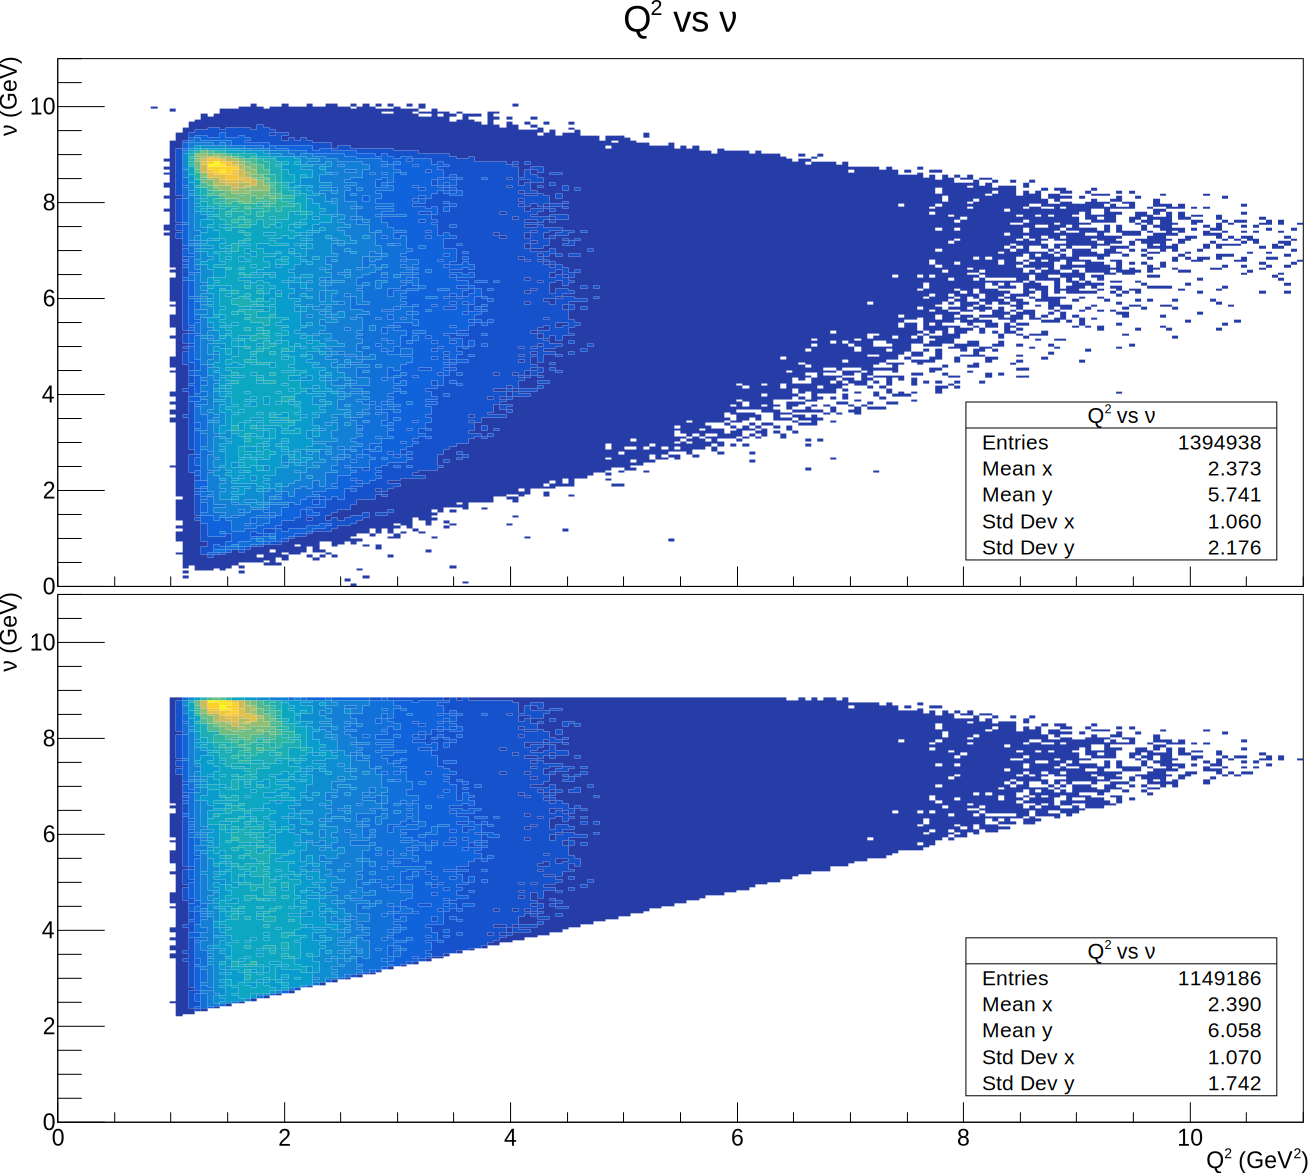
\includegraphics[width=\textwidth]{23q2_vs_nu.pdf}}
        \caption[$Q^2$ vs $\nu$ comparison]{$e^-$ $Q^2$ vs $\nu$ before and after applying the $Q^2 > 1 \text{ GeV}^2$, $W^2 > 4 \text{ GeV}^2$, and $Y_b < 0.85$ cuts, run 12016.
        Source: Own elaboration, using the \hyperlink{github.com/bleaktwig/clas12-rge-analysis}{clas12-rge-analysis} software.}
        \label{fig::q2vsnu}
    \end{figure}


    % !TEX root = ../main.tex
    \begin{figure}[b!]
        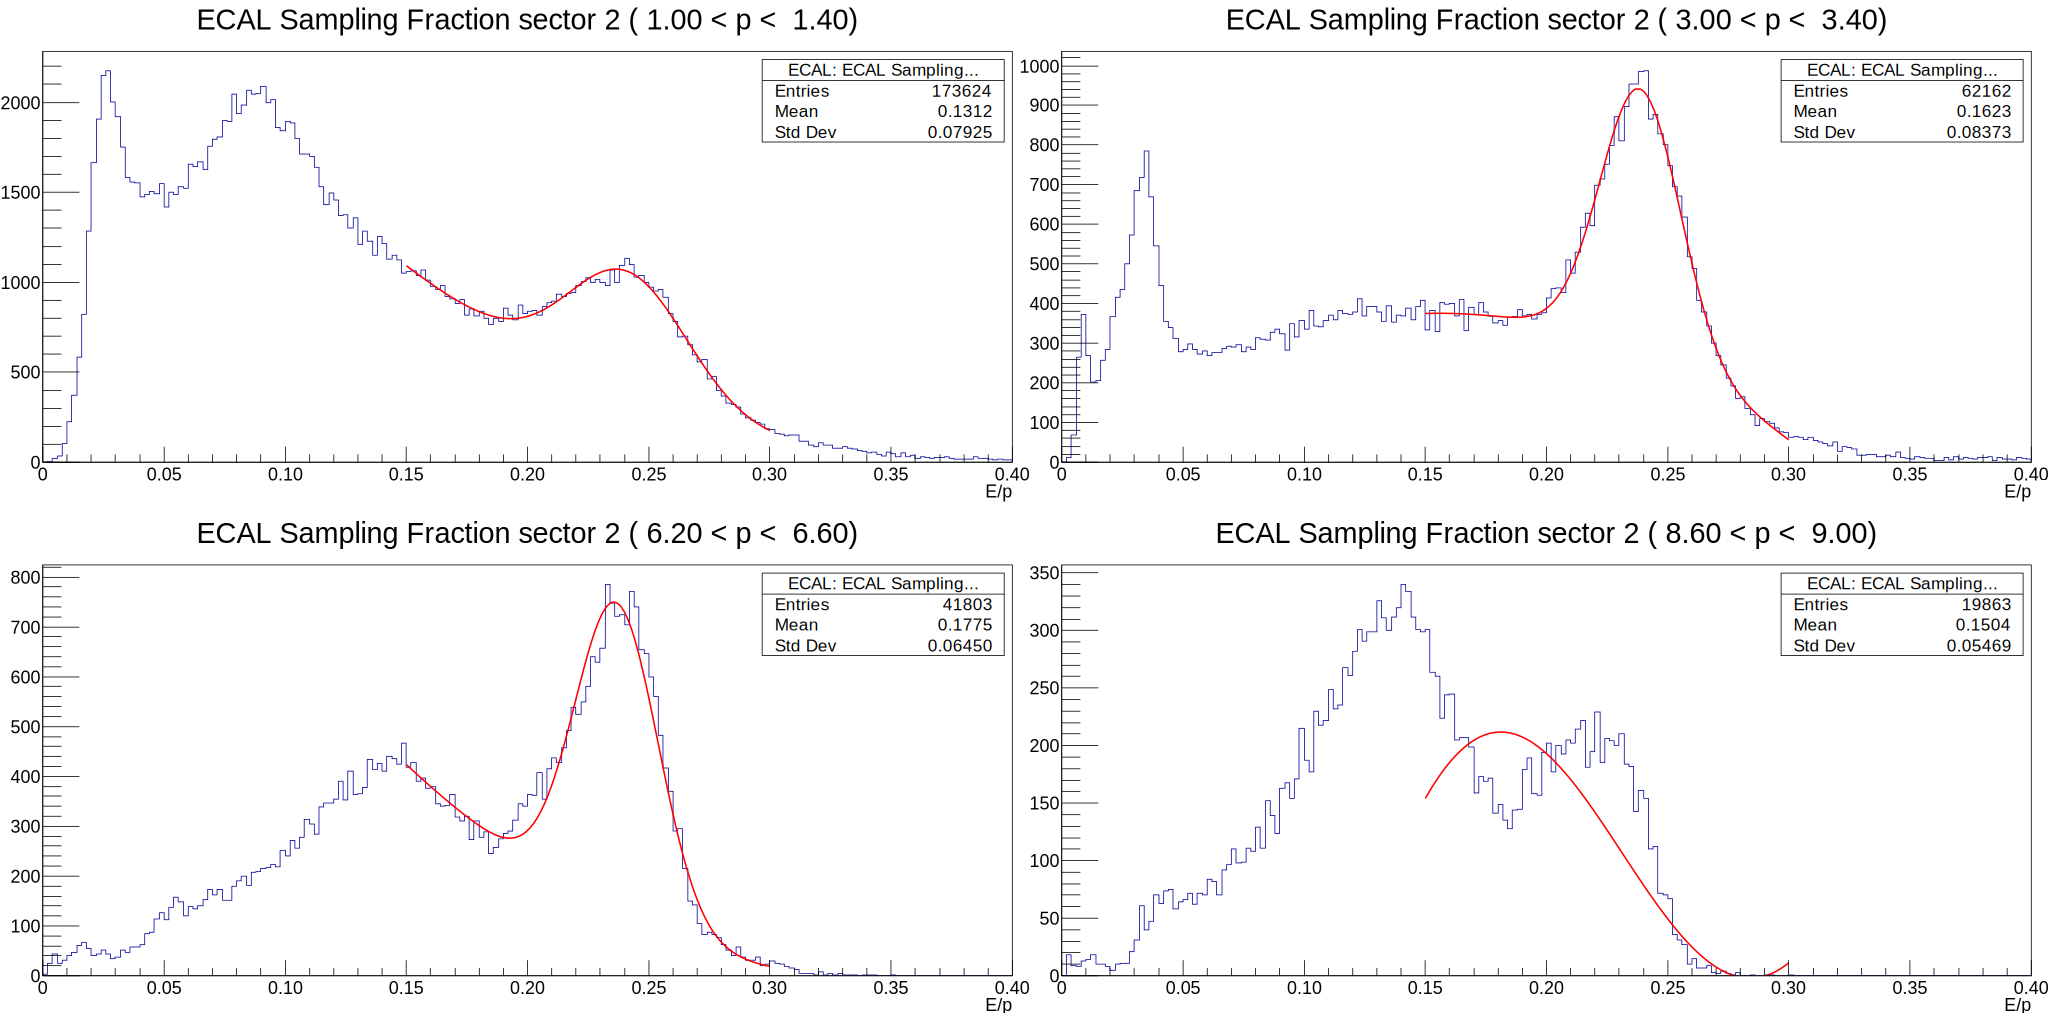
\includegraphics[width=\textwidth]{30sf_1d_plots.pdf}
        \caption[Calorimeters $E/p$ plots]
        {Four $E/p$ plots describing the sum of the deposited energy per particle on all calorimeters (PCAL, ECIN, and ECOU).
        The particles' momentum is obtained from tracking and the event builder.
        As can be seen in the northwest and the southeast plots, the corner bins -- $1.00$ to $1.40$ and $8.60$ to $9.00$ GeV respectively -- are not very reliable.}
        \floatfoot{Source: Own elaboration, using the \href{https://github.com/bleaktwig/clas12-rge-analysis}{clas12-rge-analysis} software.}
        \label{fig::13.30::sampling_fraction_fit_1d}
    \end{figure}

\subsection{Sampling Fraction}
\label{13.30::sampling_fraction}
    The energy deposited by electrons in the active area of the calorimeters is a fraction of their total energy, $E_\text{tot}$.
    This value is proportional to their momentum, $P$, for energies above a few hundred MeV.
    Heavier particles, due to their reduced penetration capabilities, tend to lose an amount of energy independent of their momentum.
    The electron sampling fraction measures the amount of energy lost depending on the momentum of a particle.
    This allows for both the measurement of the electron's energy and the differentiation of electrons from other particles \cite{wigmans2000}.

    To obtain the sampling fraction, the hits of each calorimeter by itself (PCAL, ECIN, and ECOU) are separated into arrays, with an additional array containing the union of the other three.
    Then, these arrays of hits are separated into 20 momentum bins.
    Each bin has a size of 0.4 GeV, starting at 1.0 GeV and ending at 9.0 GeV.

    1-dimensional histograms are then created from the data in these arrays, measuring the deposited energy divided by the vertex momentum ($E/p$).
    A Gaussian fit plus a quadratic background is then applied, following the function described as

    \begin{equation*}
        f(x) = p_0 g(x, \mu, \sigma) + p_1 x^2 + p_2 x + p_3, \hspace{12pt}
        \text{where} \hspace{4pt}
        g(x, \mu, \sigma) = \frac{1}{\sigma \sqrt{2\pi}} \exp \left(-\frac{1}{2} \frac{(x - \mu)^2}{\sigma^2}\right),
    \end{equation*}

    where $\mu$ and $\sigma$ represent the mean and standard deviation of the distribution, respectively. The fit is limited to the range between $0.15$ and $0.30$ for the expected $E/p$ values for electrons based on theory.

    Examples of these plots are shown in Figure \ref{fig::13.30::sampling_fraction_fit_1d}.
    From the figure, it can be observed that there are not enough electrons in the extreme momentum ranges, such as from $1$ to $1.4$ GeV or from $8.6$ to $9$ GeV.
    Consequently, the sampling fraction fit, described in Equation \eqref{eq::13.30::sampling_fraction_fit_2d}, only considers data within the range of $1.4$ to $8.6$ GeV.

    The mean of each of these fits is then extracted to serve as data points for a sampling fraction fit.
    A polynomial fit is employed since it effectively captures the shape of these points and aligns with the reconstruction software.
    The fit is described as

    \begin{equation} \label{eq::13.30::sampling_fraction_fit_2d}
        f(x) = p_0 \cdot \left(p_1 + \frac{p_2}{x} + \frac{p_3}{x^2}\right).
    \end{equation}

    The $E/p$ distribution vs $p$ is depicted in Figure \ref{fig::13.30::sampling_fraction_fit_2d}, together with this fit.

    \begin{figure}[t!]
        \includegraphics[width=\textwidth]{30sf_2d_plot.pdf}
        \caption[Calorimeters $p vs E/p$ plots]
        {A 2D plot showing momentum $p$ vs deposited energy divided by momentum $E/p$.
        The particle's deposited energy on all calorimeters is measured.
        Its momentum is obtained from tracking and the event builder.
        The fit follows the deposited energy of electrons to find their sampling fraction.}
        \floatfoot{Source: Own elaboration, using the \href{https://github.com/bleaktwig/clas12-rge-analysis}{clas12-rge-analysis} software.}
        \label{fig::13.30::sampling_fraction_fit_2d}
    \end{figure}

    Finally, the parameters of the fit are saved in plain text files, following the convention used in the CCDB.
    These parameters can be utilised later for particle identification purposes, specifically for electrons and photons.
    Furthermore, they are employed to determine the energy of electrons and photons since, as mentioned previously, not all of their energy is deposited in the calorimeters.

    % !TEX root = ../main.tex
\subsection{Acceptance Correction}
\label{13.40::acceptance_correction}
% --+ What is acceptance +------------------------------------------------------
    When discussing radiation detection, it is customary to distinguish between two types of efficiency: absolute efficiency and intrinsic detection efficiency.
    The former is defined as the fraction of events emitted by the source that are actually detected by the detector, expressed as
    \begin{equation*}
        \xi_\text{tot} = \frac{\text{events registered}}{\text{events emitted by source}}.
    \end{equation*}

    This efficiency is influenced by the detector's geometry and the probability of an interaction occurring within the detector.
    The total efficiency is also referred to as the detector acceptance.

    The total efficiency can be further decomposed into two components: the intrinsic efficiency, $\xi_{\text{int}}$, and the geometric efficiency, $\xi_{\text{geom}}$.
    The total efficiency is then given by
    \begin{equation*}
        \xi_\text{tot} = \xi_\text{int} \cdot \xi_\text{geom}.
    \end{equation*}

    The intrinsic efficiency represents the fraction of events that actually reach and are detected by the detector
    \begin{equation*}
        \xi_\text{int} = \frac{\text{events registered}}{\text{events impinging on detector}}.
    \end{equation*}

    This probability is dependent on the interaction cross-sections of the incident radiation with the detector medium.
    The intrinsic efficiency thus varies with the type of radiation, its energy, and the detector material \cite{leo1987}.

% --+ Acceptance correction through generation + simulation +-------------------
    Acceptance correction involves compensating for the total efficiency of the detector.
    To estimate this detector efficiency, a comparison is made between the total number of generated events, denoted as $N_\text{thrown}$, and the number of accepted events in a simulation of the detector, denoted as $N_\text{simul}$.
    This allows us to calculate an estimation of the detector efficiency, represented by $\tilde\xi_\text{tot}$, using
    \begin{equation*}
        \tilde\xi_\text{tot} = \frac{N_\text{simul}}{N_\text{thrown}}.
    \end{equation*}

    Naturally, the value of $\tilde\xi_\text{tot}$ is influenced by the accuracy and reliability of the event generator and simulation programs employed in the study.

% --+ Chosen bins +-------------------------------------------------------------
    The acceptance of the detector exhibits variations across the phase space of the kinematic variables.
    Therefore, in order to achieve accurate acceptance correction, the ratio $\tilde\xi_\text{tot}$ needs to be divided into bins in a five-dimensional space.
    These bins correspond to the five variables under investigation: $Q^2$, $\nu$, $z_h$, $p_T^2$, and $\phi_{PQ}$.
    To simplify the analysis process and facilitate interpretation of the results, it is advantageous to have bins of the same size for each variable.

    \pagebreak

    \begin{itemize}
        \item
            For $Q^2$, given by Equation \eqref{eq::13.23::q2}, the lower edge of the binning is defined as $1 \text{ GeV}^2$, considering that a DIS cut of $Q^2 > 1$ is applied, as described in Section \ref{13.23::dis_cuts}.
            The upper edge is defined as $11 \text{ GeV}^2$, and the bin size is set to $1 \text{ GeV}^2$ to ensure sufficient statistics per bin.
            This results in 10 bins for $Q^2$.

        \item
            As shown in Figure \ref{fig::13.23::q2_vs_nu}, the minimum value of $\nu$ (described by Equation \eqref{eq::13.23::nu}) is $2 \text{ GeV}$ due to the $W^2 > 4$ cut, and its maximum value is $9 \text{ GeV}$ due to the $Y_b < 0.85$ cut.
            The bin size is set to $1 \text{ GeV}$, resulting in a total of 8 bins for $\nu$.

        \item
            The fraction $z_h$ of the virtual photon energy carried by the measured hadron is described in Section \ref{10.32::production_time} and given by Equation \eqref{eq::10.32::zh}.
            For this DIS study, we are interested in the region of this fraction ranging from $0$ to $1$.
            The bin size is defined as $0.1$, resulting in 10 bins for $z_h$.

        \item
            $p_T^2$ represents the hadron's transverse momentum measured with respect to the virtual photon direction.
            For this experiment, very few hadrons are observed with $p_T^2 > 2 \text{ GeV}^2$, thus the binning range is defined from $0$ to $2 \text{ GeV}^2$.
            The bin size is set to $0.2 \text{ GeV}^2$, resulting in 10 bins for $p_T^2$.

        \item
            $\phi_{PQ}$ is the angle between the leptonic plane -- the plane where the paths of the initial and scattered electrons lie -- and the hadronic plane, which contains the virtual photon and the measured hadron.
            It is important to be cautious about the binning scheme for this variable, as some geometric effects can arise from the 6-sector geometry of the CLAS12 Forward Detector (FD), as described in Section \ref{11.210::forward_detector}.
            Hence, 13 bins are defined from $-180 \degree$ to $180 \degree$, resulting in a bin size of approximately $27.7 \degree$.
    \end{itemize}

    To calculate the acceptance, 10 million events were initially generated in deep inelastic kinematics using LEPTO, a Monte Carlo generator specifically designed for deep inelastic lepton-nucleon scattering \cite{ingelman1997}.
    Subsequently, these events were simulated under the experimental conditions of the RG-F experiment in CLAS12 using \texttt{gemc}, which is the standard tool for CLAS12 event simulation \cite{ungaro2020gemc}.
    The simulation took into account a torus field polarity of $-1$ and a solenoid field polarity of $-0.745033$.

    Finally, the simulated events were reconstructed using \texttt{coatjava}, which is the standard tool for CLAS12 event offline reconstruction \cite{ziegler2020}.
    Further details regarding the offline reconstruction process can be found in Section \ref{11.230::offline_reconstruction}.
    The outcomes of the acceptance correction procedure are discussed in Section \ref{14.20::acceptance_correction_results}.

    % 10M events.
    % 104k bins.
    % = 96 events per 5D bin.
    % integrated, from 0.77M to 1.25M per bin.


    \pagebreak

    % --+ Results and Conclusions +---------------------------------------------
    \graphicspath{{14results_and_conclusions/img}}
    % !TEX root = ../main.tex
\section{Results and Conclusions}
\label{14::results_and_conclusions}
    The FMT efficiency is discussed in the first section, including a brief study of it.
    Then, the second section delves into the acceptance correction results, based on the methodology described in Section \ref{13.40::acceptance_correction}.
    Following that, the study results are discussed in detail, and the conclusions of the study follow shortly thereafter.

    % Run configuration.
    All Figures in this section that show results for data are from RG-F run 12016.
    For this run, a gas H2 target was used.
    The beam energy was set to $10.4$ GeV, and the luminosity to $250$ nA.
    The solenoid field was set to an inbending polarity ($-0.75$), and the torus to its regular polarity of $-1$.
    The run has a total of $10,046,225$ events.

    % !TEX root = ../main.tex
\subsection{FMT Efficiency}
\label{14.10::fmt_efficiency}
    % Low FMT efficiency + list sources.
    Compared to the alignment work described in Section \ref{12::fmt_alignment_and_reconstruction}, a low FMT is observed in this analysis.
    This is evident in Figure \ref{fig::14.10::vz_012933}.
    Upon inspection, three causes can be attributed to this: the application of incorrect alignment constants, a geometry effect, and a general FMT offline reconstruction issue.

    \begin{figure}[b!]
        \centering\frame{
        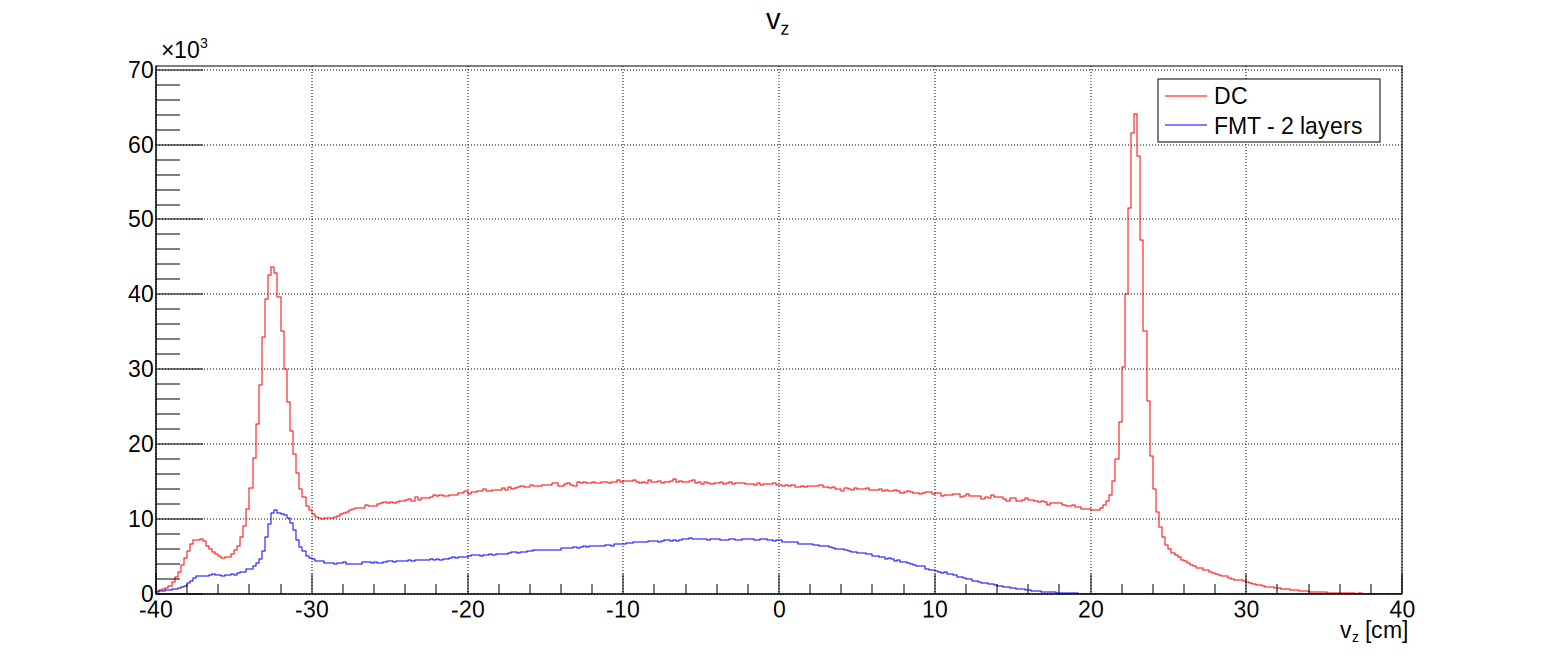
\includegraphics[width=\textwidth]{10vz_012933.pdf}}
        \caption[$v_z$ for DC and FMT, run 12933]{$v_z$ for DC (in red) and FMT (in blue). Summer 2020 data, run 12933. The wide peaks in FMT suggest an uncorrected misalignment.}
        \label{fig::14.10::vz_012933}
    \end{figure}

    In this section, we extensively discussed the efficiency of the FMT detector, addressing alignment issues, as well as the impact of implementing a geometry cut.
    The key findings can be summarized as follows: despite applying corrections, the FMT efficiency for 3-layer tracks remained low, rendering them impractical for exclusive use.
    However, by switching to Spring 2020 data and applying the geometry cut, significant improvements were observed in the detection of trigger electrons and pions.
    Moreover, we thoroughly examined the correlation between efficiency and various variables, namely $v_z$, $\theta$, $\phi$, and $p$.
    The results were as anticipated: strong correlations were observed for $v_z$ and $\theta$, while no significant correlation was found for $\phi$ or $p$.
    These findings provide valuable insights into the performance and limitations of FMT, paving the way for an acceptance correction study and the following work.

    % !TEX root = ../main.tex
\subsubsection{Alignment Effect}
\label{14.11::alignment_effect}
    % Introduction: The problem.
    The data from the RG-F experiment is divided based on the season in which the runs take place, namely Spring 2020 and Summer 2020.
    According to the run group's guidelines, it is recommended to use Summer data as it has undergone more calibration compared to the Spring data.
    However, the calibration work conducted so far does not include the FMT detector, resulting in a significant misalignment effect.

    % Cause of the problem.
    Through simple visual inspection, two distinct peaks can be clearly observed between $z = -36$ cm and $z = -30$ cm in Figure \ref{fig::12.41::dc_vs_fmt_vz_11983}.
    The leftmost peak corresponds to the scattering chamber window, while the second peak corresponds to the RG-F target window.
    These peaks appear merged in Figure \ref{fig::14.10::vz_012933}.
    As discussed in Section \ref{12::fmt_alignment_and_reconstruction}, this issue arises due to the lack of correction for FMT misalignments.

    % Solution.
    The simplest solution is to utilise Spring data.
    Although more calibration work has been performed on the Summer data, it mainly pertains to the CD, which is not used in this analysis.
    Figure \ref{fig::14.11::vz_012016} depicts the same $v_z$ plot from Spring 2020 run 12016, where both peaks are clearly visible.
    This indicates that the misalignment issue has been appropriately addressed in that particular run.

    \begin{figure}[t!]
        \centering\frame{
        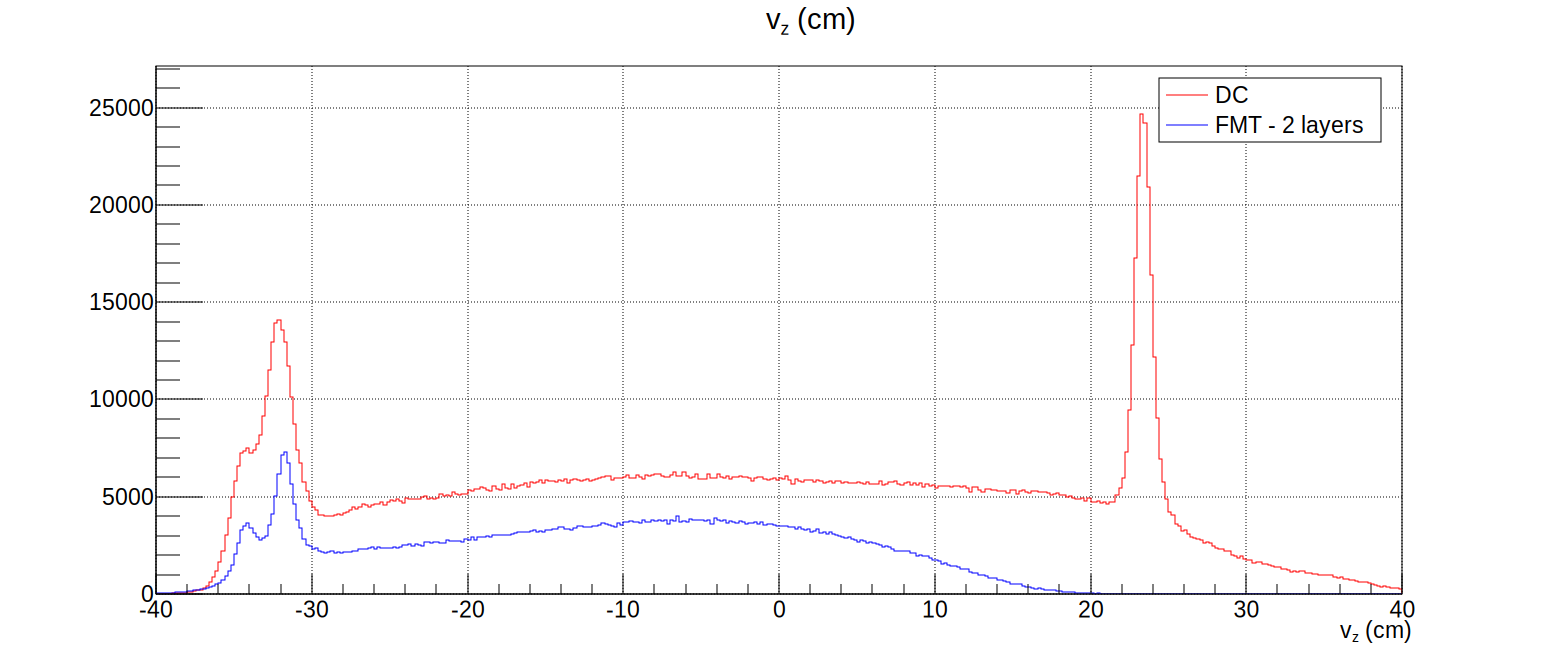
\includegraphics[width=\textwidth]{11vz_012016.pdf}}
        \caption[$v_z$ for DC and FMT, run 12016]{$v_z$ for DC (in red) and FMT (in blue).
        Spring 2020 data, run 12016. The upstream twin peaks can be clearly distinguished, suggesting a correct misalignment correction.
        Source: Own elaboration, using the \href{https://github.com/bleaktwig/clas12-rge-analysis}{clas12-rge-analysis} software.}
        \label{fig::14.11::vz_012016}
    \end{figure}

    % !TEX root = ../main.tex
\subsubsection{Geometry Effect}
\label{14.12::geometry_effect}
    % The effect has already been presented and discussed before, so we're brief.
    This problem has already been extensively discussed in section \ref{12.42::geometry_effect}.
    In summary, the FMT detector is located at approximately $z \approx 26$ cm, and it exhibits poor performance for targets located too close to it.
    The strength of this effect can be quantified by applying the geometry cut described by Equation \eqref{eq::12.42::fmt_geometry_cut} to both the DC and FMT tracks.
    Figure \ref{fig::14.12::vz_012016_geomcut} illustrates the impact of this cut on both the DC and FMT tracks when applied to figure \ref{fig::14.11::vz_012016}.
    The effect of the cut on a $v_z$ vs $\theta$ plot can be observed in Figure \ref{eq::12.42::vz_vs_theta}.

    Based on this cut and the FMT's position along the $z$-axis, subsequent plots will be confined to the range $-30 \text{cm} < v_z < 20 \text{cm}$.

    \begin{figure}[h!]
        \centering\frame{
        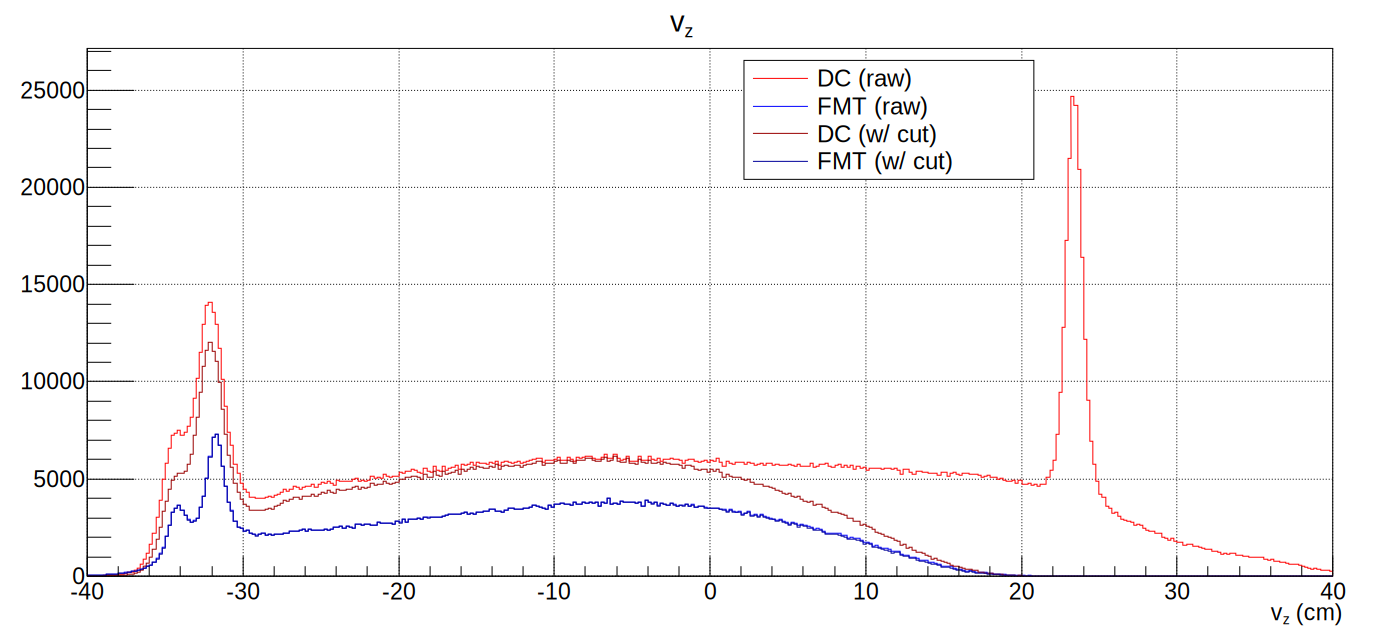
\includegraphics[width=\textwidth]{12vz_012016_geomcut.pdf}}
        \caption[$v_z$ for DC and FMT, w/ and w/out the geometry cut, run 12016]{$v_z$ for DC without the geometry cut (in red), with it (in dark red), for FMT without it (in blue), and with it (in dark blue).
        Spring 2020 data, run 12016.
        The effect is very clear on DC tracks, yet it almost doesn't affect FMT tracks.
        Source: Own elaboration, using the \hyperlink{github.com/bleaktwig/clas12-rge-analysis}{clas12-rge-analysis} software.}
        \label{fig::14.12::vz_012016_geomcut}
    \end{figure}

    % !TEX root = ../main.tex
\subsubsection{Reconstruction Effect}
\label{14.13::reconstruction_effect}
    Even after correcting for both the alignment and geometry issues, the FMT still exhibits lower efficiency compared to what was observed during alignment (compare Figure \ref{fig::14.12::vz_012016_geomcut} with Figure \ref{fig::12.43::dc_vs_fmt_vz_11983_corrected}).
    After conducting a thorough study, it was determined that this effect is not correlated with the run number, beam energy, or beam luminosity.
    Consequently, it can be concluded that the issue is not caused by hardware problems or run conditions.

    Based on these findings, the logical conclusion is that the effect stems from a general issue in the FMT offline reconstruction for data.
    Identifying and rectifying this issue would require a larger project beyond the scope of this thesis and is therefore left as future work.
    For the purposes of this analysis, we will rely on a large number of events to minimize any statistical deficiencies.

    % !TEX root = ../main.tex
\subsubsection{Efficiency Study}
\label{sssec::efficiency_study}
% --+ Integrated. +---------------------------------------------------------
    With all these effects accounted for, we can proceed to study the efficiency in detail.
    First, if we define FMT efficiency as the percentage of DC tracks that get accepted by FMT, we get table \ref{tab::fmt_efficiency_study} for runs 12933 (Summer 2020) and 12016 (Spring 2020).

    \begin{center}
        \begin{tabularx}{0.70\textwidth}{Xr|rrcrr}
            & & \multicolumn{2}{l}{\textbf{Run 12933}}  & & \multicolumn{2}{l}{\textbf{Run 12016}} \\
                             &          & raw  & w/ cut   & & raw  & w/ cut   \\
            \hline
            \textbf{$e^-$}   & 2 layers & 25.1\% & 37.5\% & & 32.7\% & 53.7\% \\
                             & 3 layers &  5.6\% &  8.5\% & &  9.9\% & 16.4\% \\
            \hline
            \textbf{$\pi^+$} & 2 layers &  6.5\% & 13.7\% & & 11.1\% & 28.0\% \\
                             & 3 layers &  0.3\% &  0.7\% & &  1.0\% &  2.7\% \\
            \hline
            \textbf{$\pi^-$} & 2 layers &  5.6\% & 14.2\% & &  8.9\% & 29.5\% \\
                             & 3 layers &  0.3\% &  0.7\% & &  0.9\% &  2.9\%
        \end{tabularx}
        \label{tab::fmt_efficiency_study}
    \end{center}

    % TODO. Change percentages based on new table.
    By switching from Summer to Spring data, we see a $\sim32\%$ increase in trigger electrons detected, and a $\sim36\%$ in all particles.
    Then, by applying the geometry cut in $v_z$ and $\theta$, $\sim64\%$ more trigger electrons are detected (for a $\sim184\%$ total increase), and $\sim126\%$ more particles in general are detected (for a $\sim207\%$ total increase).

% --+ Separated. +----------------------------------------------------------
    We can then check how the efficiency changes as result of the corrections.
    Due to the geometric cut, we expect a strong dependency on $v_z$ and $\theta$, and at most a weak one on $\phi$ and $p$.
    This is what we see in data, as is shown in figure \ref{fig::fmt_efficiencies}.

    % TODO. Explain the loss of dips in $\phi$ efficiency.

    \begin{figure}[t!]
        \centering\frame{
        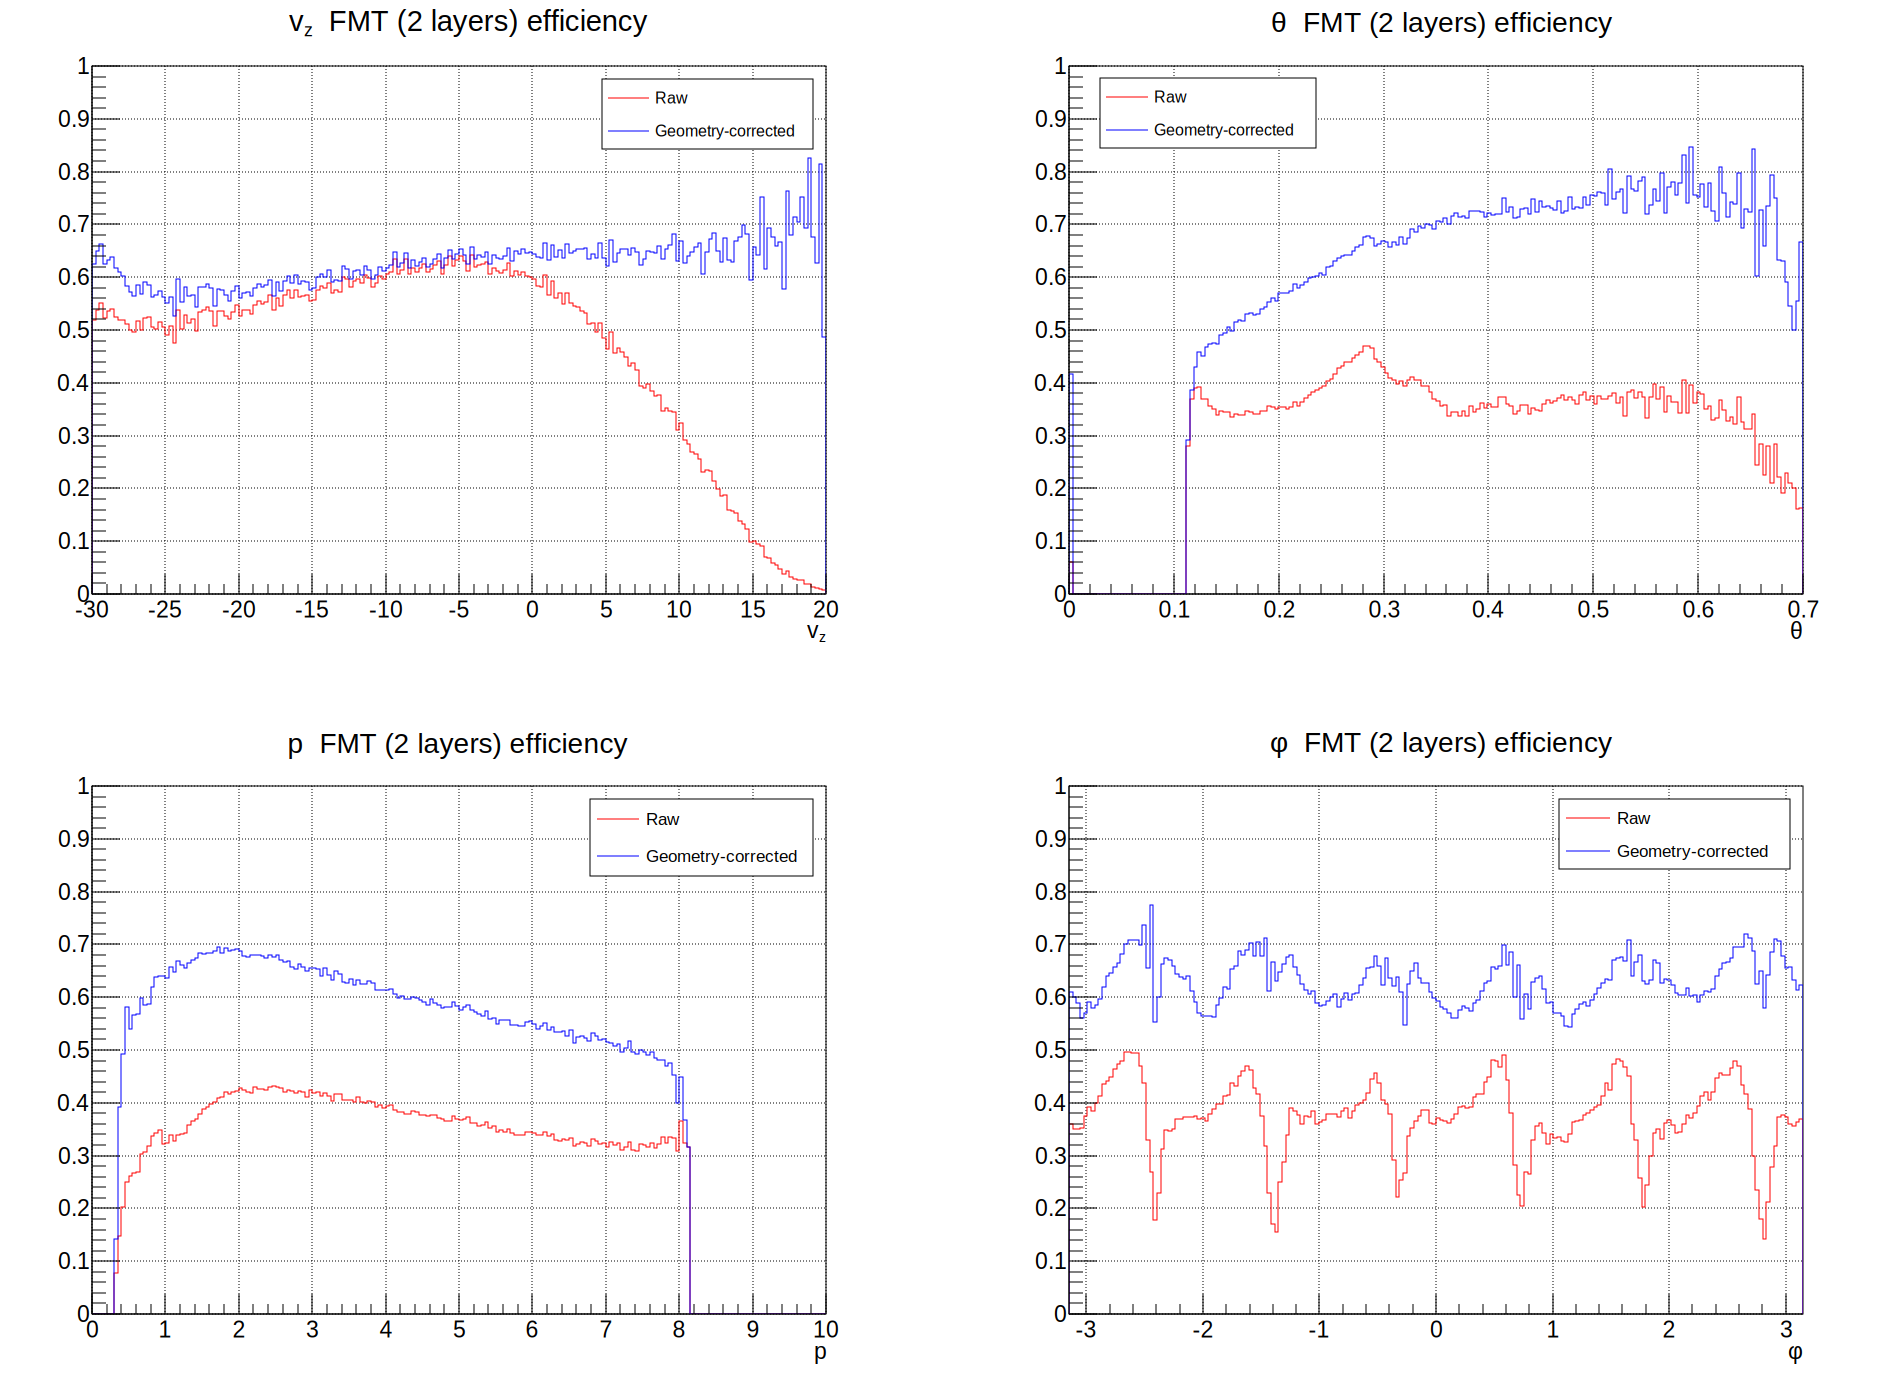
\includegraphics[width=\textwidth]{14efficiencies.pdf}}
        \caption[$v_z$, $\theta$, $\phi$, and $p$ efficiencies for FMT tracks, run 12016]{$v_z$, $\theta$, $\phi$, and $p$ efficiencies for FMT tracks. FMT Efficiency is defined as the percentage of DC tracks that are detected by 2 FMT layers. Run 12016.}
        \label{fig::fmt_efficiencies}
    \end{figure}


    % !TEX root = ../main.tex
\subsection{Acceptance Correction Results}
\label{14.20::acceptance_correction_results}
    DC and FMT acceptances were obtained by following the procedure described in Section \ref{13.13::acc_corr}.
    In this section, we will study the acceptance percentage for each electron and hadronic variable.
    These numbers represent the percentage of thrown particles that were detected by the DC and by 2 or 3 FMT layers in addition to DC in the GEMC simulation.

    Since they represent the acceptance percentage, all plots display a calculated division as follows
    \begin{equation}
        y_\text{acc} = \frac{y_r}{y_t},
        \label{eq::14.20::acc}
    \end{equation}
    where $y_\text{acc}$ is the percentage of accepted particles, $y_r$ is the number of reconstructed particles by the studied detector in the GEMC simulation, and $y_t$ is the number of particles thrown by LEPTO.

    Then, to propagate the error of $y_r$ ($e_d$) and $y_t$ ($e_t$) to $y_\text{acc}$ ($e_\text{acc}$), we have
    \begin{align}
        e_\text{acc} &= \delta \left(\frac{y_r}{y_t}\right)
        \nonumber \\
        &= y_\text{acc} \cdot \sqrt{
            \left( \frac{e_r}{y_r} \right)^2 + \left( \frac{e_t}{y_t} \right)^2
        },
        \nonumber
        \intertext{since $y_t$ is the number of trials, we can assume $e_t = 0$, and thus}
        &= y_\text{acc} \cdot \frac{e_r}{y_r}.
        \label{eq::14.20::acc_error_estimation}
    \end{align}

    From the Central Limit Theorem, assuming a normal distribution, the variance $e_r^2$ is given by
    \begin{equation*}
        e_r^2 = y_t \cdot y_\text{acc} (1 - y_\text{acc}).
    \end{equation*}

    Replacing this in Equation \eqref{eq::14.20::acc_error_estimation}, we obtain
    \begin{equation*}
        e_\text{acc} = y_\text{acc} \cdot \frac{\sqrt{y_t y_\text{acc}(1 - y_\text{acc})}}{y_r}.
    \end{equation*}

    Now, replacing $y_\text{acc}$ with its definition from Equation \eqref{eq::14.20::acc}, we arrive at the final error expression
    \begin{equation}
        e_\text{acc} = \sqrt{\frac{y_\text{acc}(1-y_\text{acc})}{y_t}}.
        \label{eq::14.20::acc_error}
    \end{equation}

    % !TEX root = ../main.tex
\subsubsection{Electron Variables}
\label{14.21::electron_variables}
    First, we'll study the $Q^2$ and $\nu$ acceptances for the scattered $e^-$.
    $Q^2$ and $\nu$ acceptances are presented in Figure \ref{fig::14.21::electron_acc}.
    Each one is presented in integrated kinematical region for the other variable.

    \textbf{TODO. Say something?}



    \begin{figure}
        \centering
        % Q2.
        \begin{subfigure}[b]{0.49\textwidth}
            \centering
            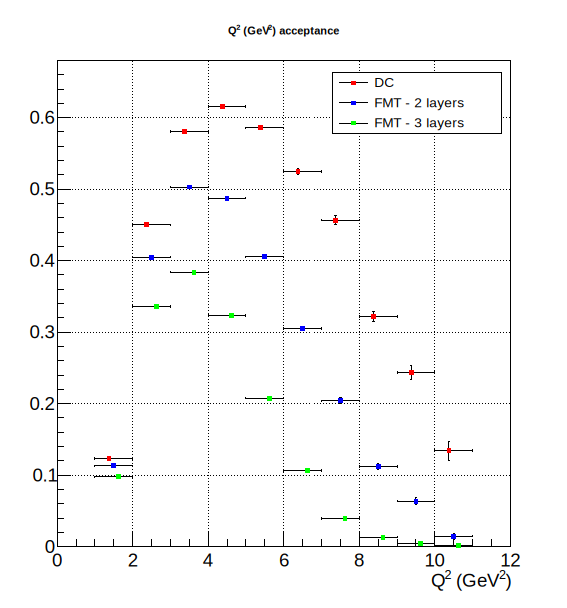
\includegraphics[width=\textwidth]{21q2_acc.pdf}
            \caption{$Q^2$ acceptance.}
            \label{fig::14.21::q2_acc}
        \end{subfigure}
        \hfill
        % nu.
        \begin{subfigure}[b]{0.49\textwidth}
            \centering
            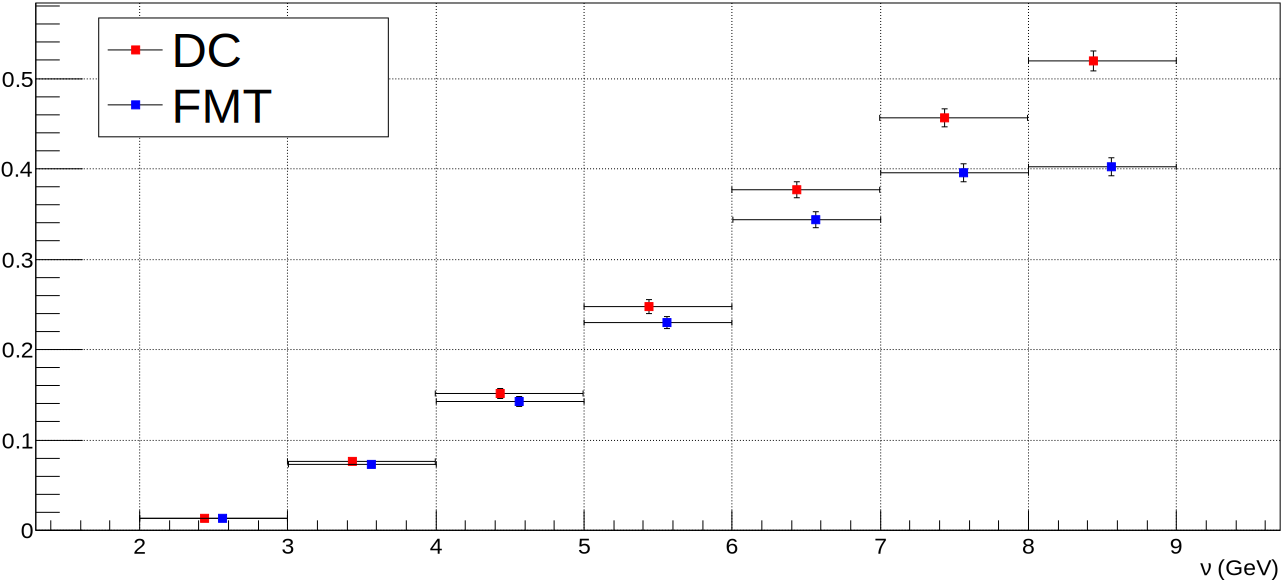
\includegraphics[width=\textwidth]{21nu_acc.pdf}
            \caption{$\nu$ acceptance.}
            \label{fig::14.21::nu_acc}
        \end{subfigure}
        \caption[Electron variables acceptance.]{Electron variables acceptance.
        $\nu$ is integrated in \ref{fig::14.21::q2_acc}, and $Q^2$ is integrated in \ref{fig::14.21::nu_acc}.
        The bin markers are slightly shifted in $x$ to improve legibility.
        Source: Own elaboration, using the \href{https://github.com/bleaktwig/clas12-rge-analysis}{clas12-rge-analysis} software.}
        \label{fig::14.21::electron_acc}
    \end{figure}

    % !TEX root = ../main.tex
\subsubsection{Hadronic Variables}
\label{14.22::hadronic_variables}
    The acceptance of the hadronic variables $z_h$, $p_T^2$, and $\phi_{PQ}$ for $e^-\pi^+$ and $e^-\pi^-$ are presented in Figure \ref{fig::14.22::hadronic_acc}.
    Each one is presented in integrated kinematical region for all electron variables and other hadronic variables.

    % Lower acceptance.
    It's worth noting that these acceptances are lower than those for electron variables.
    This is to be expected, since they require both the trigger electron and at least one hadron to be accepted by the detector.
    This same effect is seen in the $e^-\pi^+$ and $e^-\pi^-$ entries presented in the efficiency Table \ref{tab::14.14::fmt_efficiency_study}.

    % Particle charge-dependent acceptance.
    % TODO. Add phi vs theta (positive particles) plot and explain the difference in acceptances between pi+ and pi- based on that.

    \begin{figure}
        \centering
        % zh pi+.
        \begin{subfigure}[b]{0.49\textwidth}
            \centering
            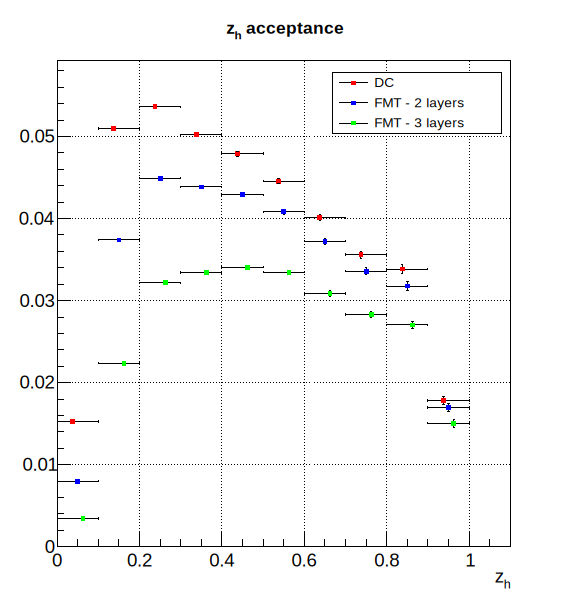
\includegraphics[width=\textwidth]{22zh_acc_211.pdf}
            \caption{$z_h$ acceptance for $e^-\pi^+$.}
            \label{fig::14.22::zh_acc_211}
        \end{subfigure}
        \hfill
        % zh pi-.
        \begin{subfigure}[b]{0.49\textwidth}
            \centering
            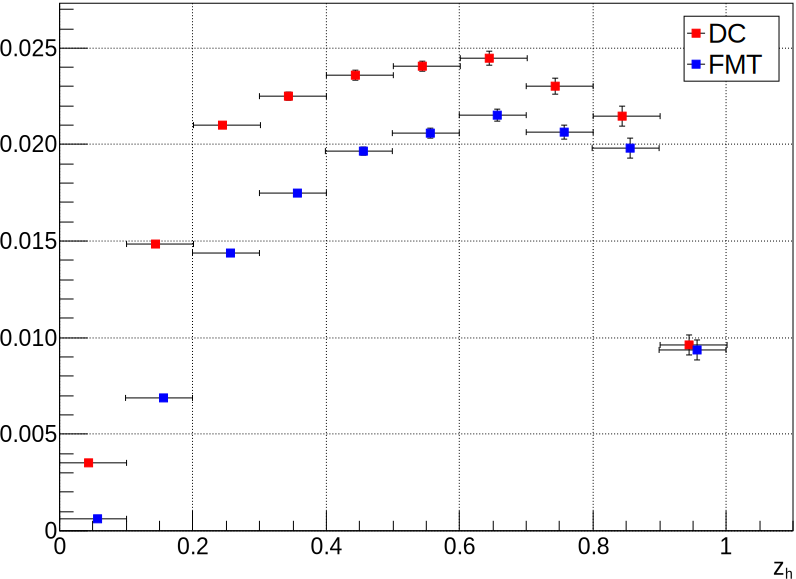
\includegraphics[width=\textwidth]{22zh_acc_-211.pdf}
            \caption{$z_h$ acceptance for $e^-\pi^-$.}
            \label{fig::14.22::zh_acc_-211}
        \end{subfigure}

        \centering
        % pt2 pi+.
        \begin{subfigure}[b]{0.49\textwidth}
            \centering
            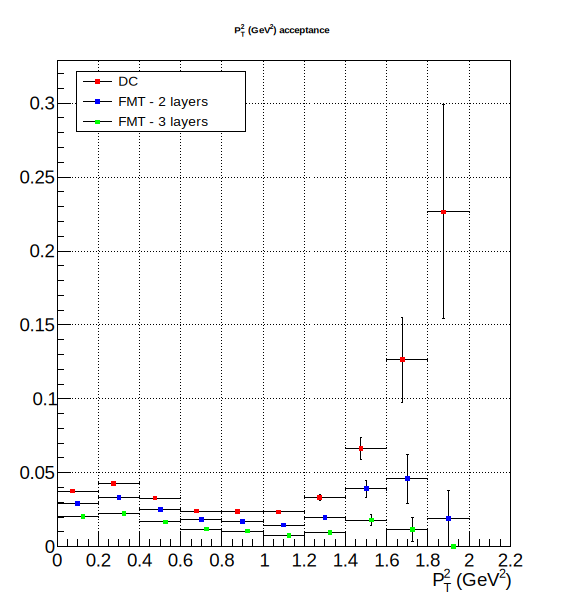
\includegraphics[width=\textwidth]{22pt2_acc_211.pdf}
            \caption{$p_T^2$ acceptance for $e^-\pi^+$.}
            \label{fig::14.22::pt2_acc_211}
        \end{subfigure}
        \hfill
        % pt2 pi-.
        \begin{subfigure}[b]{0.49\textwidth}
            \centering
            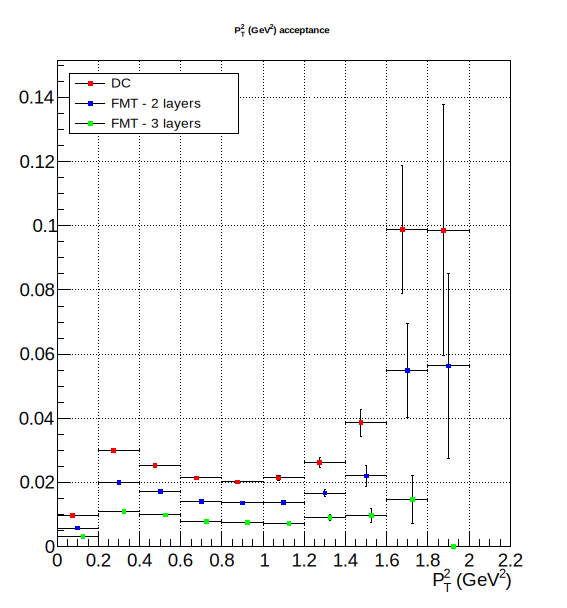
\includegraphics[width=\textwidth]{22pt2_acc_-211.pdf}
            \caption{$p_T^2$ acceptance for $e^-\pi^-$.}
            \label{fig::14.22::pt2_acc_-211}
        \end{subfigure}

        \centering
        % phipq pi+.
        \begin{subfigure}[b]{0.49\textwidth}
            \centering
            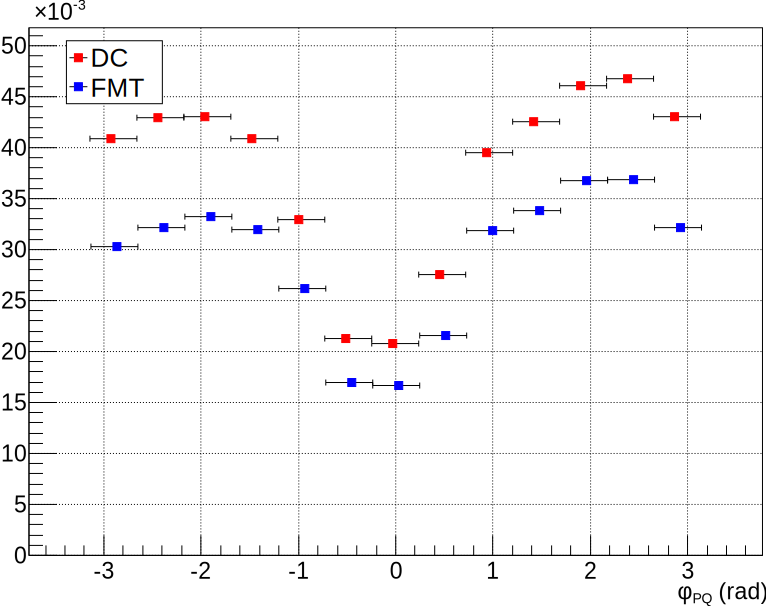
\includegraphics[width=\textwidth]{22phipq_acc_211.pdf}
            \caption{$\phi_{PQ}$ acceptance for $e^-\pi^+$.}
            \label{fig::14.22::phipq_acc_211}
        \end{subfigure}
        \hfill
        % phipq pi-.
        \begin{subfigure}[b]{0.49\textwidth}
            \centering
            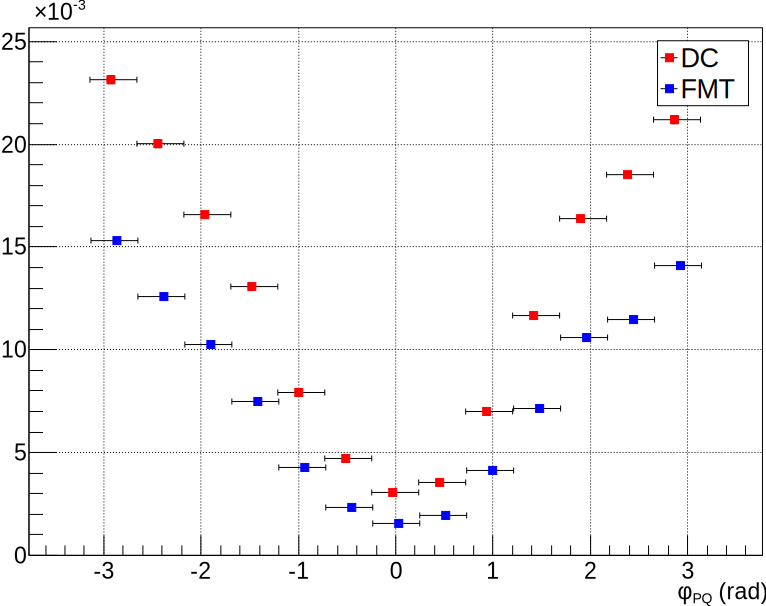
\includegraphics[width=\textwidth]{22phipq_acc_-211.pdf}
            \caption{$\phi_{PQ}$ acceptance for $e^-\pi^-$.}
            \label{fig::14.22::phipq_acc_-211}
        \end{subfigure}
        \caption[hadronic variables acceptance]
        {$z_h$, $p_T^2$, and $\phi_{PQ}$ acceptances for $e^-\pi^+$ and $e^-\pi^-$.
        All electron and other hadronic variables are integrated in all Figures.
        The bin markers are slightly shifted in $x$ to improve legibility.}
        \floatfoot{Source: Own elaboration, using the \href{https://github.com/bleaktwig/clas12-rge-analysis}{clas12-rge-analysis} software.}
        \label{fig::14.22::hadronic_acc}
    \end{figure}


    % !TEX root = ../main.tex
\subsection{Study Results}
\label{14.30::study_results}
    % Explain binning scheme selected.
    To select a region in $v_z$ to place the RG-E target, two criteria were considered: a phase space study and a statistics study.
    In the phase space study, the RG-F target gas region ($-30 < v_z < 20$ cm) was divided into ten 5 cm bins, and the phase space of each kinematic variable was analysed in each bin.
    The results of this study are presented in Section \ref{14.31::phase_space_study}.
    For the statistics study, the region chosen in the phase space study was further divided into 1 cm bins.
    The study aimed to determine which 7 cm region within the chosen range had the largest statistics.
    The validity of this choice was evaluated using a gemc simulation of the RG-E target system.
    The results of this study are presented in Section \ref{14.32::statistics_study}.

    % Statistical error estimation.
    Regarding the statistical error estimation, the total statistical error on the acceptance-corrected result, denoted as $e_\text{corr}$, needs to consider both the statistical error of the measurements ($e_\text{meas}$) and the acceptance correction ($e_\text{acc}$).
    The statistical error of the measurements, $e_\text{meas}$, is purely statistical in nature and is given by
    \begin{equation*}
        e_\text{meas} = \frac{\delta y_\text{meas}}{y_\text{meas}},
    \end{equation*}
    The acceptance correction error, $e_\text{acc}$, was derived in Equation \eqref{eq::14.20::acc_error}.

    Since $e_\text{meas}$ arises purely from experimental data and $e_\text{acc}$ is purely from simulation, they are considered to be completely uncorrelated.
    Therefore, the total statistical error of the acceptance-corrected result can be estimated as the quadratic addition of the two errors, i.e.,
    \begin{equation*}
        e_\text{corr} = \sqrt{e_\text{meas}^2 + e_\text{acc}^2}.
    \end{equation*}

    % !TEX root = ../main.tex
\subsubsection{Phase Space Study}
\label{14.31::phase_space_study}
    % Introduction.
    Considering the objectives of this DIS study, it is advantageous to maximise the phase space of each kinematic variable of study.
    This approach broadens the scope of investigation, increases sensitivity to detect rare phenomena, and facilitates the testing of theoretical predictions for future studies using the double target system.
    Therefore, the first criterion for selecting a $v_z$ region for the target is to find a region that provides the maximum range of kinematic variables.

    % Resulting plots.
    The resulting plots show the acceptance-corrected DIS variables separated into $v_z$ bins.
    Figures \ref{fig::14.31::q2_vz} and \ref{fig::14.31::nu_vz} display the distributions of the electron variables $Q^2$ and $\nu$, respectively.
    The $z_h$ distributions for $e^-\pi^+$ and $e^-\pi^-$ can be observed in Figures \ref{fig::14.31::zh_211_vz} and \ref{fig::14.31::zh_-211_vz}, respectively.
    Figures \ref{fig::14.31::pt2_211_vz} and \ref{fig::14.31::pt2_-211_vz} show the distributions of $p_T^2$ for $e^-\pi^+$ and $e^-\pi^-$, respectively.
    Finally, Figures \ref{fig::14.31::phipq_211_vz} and \ref{fig::14.31::phipq_-211_vz} present the distributions of $\phi_{PQ}$ for $e^-\pi^+$ and $e^-\pi^-$, respectively.
    These plots provide insights into the dependence of each DIS variable on the $v_z$ coordinate.
    For these same distributions without acceptance correction, please see Appendix \ref{20.04::dis_vz_plots}.

    % Q2.
    In the study of $Q^2$, as shown in Figure \ref{fig::14.31::q2_vz}, the higher end of the variable's phase space is limited for $v_z < -5$ cm, with the effect becoming more pronounced as we move further upstream.
    This effect can be understood by considering the compounded effect of the $\theta$ efficiency for negative particles (as seen in Figure \ref{fig::14.21::theta_study_neg}) and the limited acceptance region of FMT (described by Equation \eqref{eq::12.42::fmt_geometry_cut} and illustrated in Figure \ref{eq::12.42::vz_vs_theta}).

    The higher end of $\theta$ becomes limited for lower $v_z$ values.
    Based on the objective of maximising the phase space of each variable, this suggests setting the minimum $v_z$ for the RG-E target near $-5$ cm.
    Additionally, it is noted that the variable exhibits an unusual shape for $10$ cm $< v_z < 20$ cm, likely due to the cut in low $\theta$ angles in that region, which is another consequence of the FMT acceptance region.

    % nu.
    In the study of $\nu$, as seen in Figure \ref{fig::14.31::nu_vz}, it was previously observed that $\nu$ has no direct correlation with the scattering angle $\theta_C$ (Section \ref{14.20::acceptance_correction_results}).
    Therefore, no significant effect on the phase space of $\nu$ is observed for $v_z < -5$ cm, unlike $Q^2$.
    However, a loss is observed in the lower end of the phase space for $v_z = 10$ cm and downstream.
    Based on this effect, it is reasonable to keep $v_z$ below approximately 10 cm to preserve the largest possible phase space of $\nu$.

    % zh.
    In the study of $z_h$, despite its lack of direct correlation with the electron's and pion's $\theta$, clear differences are observed across different $v_z$ bins, as shown in Figures \ref{fig::14.31::zh_211_vz} and \ref{fig::14.31::zh_-211_vz}.
    However, this can be explained by its inverse correlation with $\nu$ (as described in Equation \eqref{eq::10.32::zh}).
    Similar to $\nu$, the extreme phase space loss is primarily observed for $v_z > 10$ cm, and therefore, no additional severe restrictions on the $v_z$ region are imposed beyond those defined based on the studies of $Q^2$ and $\nu$.

    % pt2.
    In the study of $p_T^2$, as depicted in Figures \ref{fig::14.31::pt2_211_vz} and \ref{fig::14.31::pt2_-211_vz}, large statistical fluctuations are observed for $p_T^2 > 1.4 \text{GeV}^2$, consistent with the prediction in Section \ref{14.22::hadronic_variables}.
    Studying the phase space of the variable, a cutoff at high $p_T^2$ values is observed for $v_z < -5$ cm and $v_z > 15$ cm, similar to what was seen for $Q^2$.
    Based on this observation, no additional restrictions are imposed on the $v_z$ region under study.

    % phipq.
    Regarding the study of $\phi_{PQ}$, as shown in Figures \ref{fig::14.31::phipq_211_vz} and \ref{fig::14.31::phipq_-211_vz}, no easily discernible loss is observed in the phase space of $\phi_{PQ}$ as we vary $v_z$.
    While there are significant changes in the shape of the variable distribution across different $v_z$ bins, conducting a detailed shape study is beyond the scope of this thesis, as ample information is already provided by the other DIS variables.

    % !TEX root = ../main.tex
\subsubsection{Statistics Study}
\label{14.32::statistics_study}
    After obtaining the $v_z$ region with the maximum range of kinematic variables, our second criterion is to maximise statistics inside this region.
    With phase space already maximised, this allows us to increase the statistical precision of future studies, enabling a thorough exploration of the parameter space.

    Based on the results of the different phase space studies, we'll limit the scope of this statistics study to the region $-5 \text{cm} < v_z < 10 \text{cm}$, the result of which can be observed in Figure \ref{fig::14.32::statistics}.
    The objective of this study is to find the 7 cm region in $v_z$ with the highest statistics.
    The choice of 7 cm in particular comes from the length of the double target, where the liquid target has a length of 3 cm, the separation between the liquid and solid target is 4 cm, and the solid target is of negligible width for the scope of this study.

    First, we look at $e^-$ statistics, seen in Figure \ref{fig::14.32::statistics_11}.
    It is trivial to note that, in the studied range, the more upstream we look, the more statistics are seen.
    Therefore, the best region for the placement of the target is from $-5$ to $2$ cm.
    This result is only reinforced by the results observed in $e^-\pi^+$ and $e^-\pi^-$ statistics, which can be seen in Figures \ref{fig::14.32::statistics_211} and \ref{fig::14.32::statistics_-211}.

    % statistics.
    \begin{figure}
        \centering
        % e-.
        \begin{subfigure}[b]{\textwidth}
            \centering
            \includegraphics[width=\textwidth]{32statistics_11.png}
            \caption{$e^-$ statistics.}
            \label{fig::14.32::statistics_11}
        \end{subfigure}
        \centering
        % e-pi+.
        \begin{subfigure}[b]{0.49\textwidth}
            \centering
            \includegraphics[width=\textwidth]{32statistics_211.png}
            \caption{$e^-\pi^+$ statistics.}
            \label{fig::14.32::statistics_211}
        \end{subfigure}
        \hfill
        % e-pi-.
        \begin{subfigure}[b]{0.49\textwidth}
            \centering
            \includegraphics[width=\textwidth]{32statistics_-211.png}
            \caption{$e^-\pi^-$ statistics.}
            \label{fig::14.32::statistics_-211}
        \end{subfigure}
        \caption[Statistics for $e^-$, $e^-\pi^+$, and $e^-\pi^-$ against $v_z$]
        {$e^-$, $e^-\pi^+$, and $e^-\pi^-$ statistics against $v_z$ for run 12016.
        No acceptance correction was applied to these results.}
        \floatfoot{Source: Own elaboration, using the \href{https://github.com/bleaktwig/clas12-rge-analysis}{clas12-rge-analysis} software.}
        \label{fig::14.32::statistics}
    \end{figure}


    % Q2.
    \begin{figure}
        \centering
        \includegraphics[width=\textwidth]{31q2_vz.png}
        \caption[Acceptance-corrected $Q^2$ separated in $v_z$ bins]
        {Acceptance-corrected $Q^2$ detected by DC and FMT, separated in $v_z$ bins.
        Run 12016.
        The bin markers are slightly shifted in $x$ to improve legibility.}
        \floatfoot{Source: Own elaboration, using the \href{https://github.com/bleaktwig/clas12-rge-analysis}{clas12-rge-analysis} software.}
        \label{fig::14.31::q2_vz}
    \end{figure}

    % nu.
    \begin{figure}
        \centering
        \includegraphics[width=\textwidth]{31nu_vz.png}
        \caption[Acceptance-corrected $\nu$ separated in $v_z$ bins]
        {Acceptance-corrected $\nu$ detected by DC and FMT, separated in $v_z$ bins.
        Run 12016.
        The bin markers are slightly shifted in $x$ to improve legibility.}
        \floatfoot{Source: Own elaboration, using the \href{https://github.com/bleaktwig/clas12-rge-analysis}{clas12-rge-analysis} software.}
        \label{fig::14.31::nu_vz}
    \end{figure}

    % zh.
    \begin{figure}
        \centering
        \includegraphics[width=\textwidth]{31zh_vz_211.png}
        \caption[Acceptance-corrected $z_h$ for $e^-\pi^+$ separated in $v_z$ bins]
        {Acceptance-corrected $z_h$ for $e^-\pi^+$ detected by DC and FMT, separated in $v_z$ bins.
        Run 12016.
        The bin markers are slightly shifted in $x$ to improve legibility.}
        \floatfoot{Source: Own elaboration, using the \href{https://github.com/bleaktwig/clas12-rge-analysis}{clas12-rge-analysis} software.}
        \label{fig::14.31::zh_211_vz}
    \end{figure}

    \begin{figure}
        \centering
        \includegraphics[width=\textwidth]{31zh_vz_-211.png}
        \caption[Acceptance-corrected $z_h$ for $e^-\pi^-$ separated in $v_z$ bins]
        {Acceptance-corrected $z_h$ for $e^-\pi^-$ detected by DC and FMT, separated in $v_z$ bins.
        Run 12016.
        The bin markers are slightly shifted in $x$ to improve legibility.}
        \floatfoot{Source: Own elaboration, using the \href{https://github.com/bleaktwig/clas12-rge-analysis}{clas12-rge-analysis} software.}
        \label{fig::14.31::zh_-211_vz}
    \end{figure}

    % pt2.
    \begin{figure}
        \centering
        \includegraphics[width=\textwidth]{31pt2_vz_211.png}
        \caption[Acceptance-corrected $p_T^2$ for $e^-\pi^+$ separated in $v_z$ bins]
        {Acceptance-corrected $p_T^2$ for $e^-\pi^+$ detected by DC and FMT, separated in $v_z$ bins.
        Run 12016.
        The bin markers are slightly shifted in $x$ to improve legibility.}
        \floatfoot{Source: Own elaboration, using the \href{https://github.com/bleaktwig/clas12-rge-analysis}{clas12-rge-analysis} software.}
        \label{fig::14.31::pt2_211_vz}
    \end{figure}

    \begin{figure}
        \centering
        \includegraphics[width=\textwidth]{31pt2_vz_-211.png}
        \caption[Acceptance-corrected $p_T^2$ for $e^-\pi^-$ separated in $v_z$ bins]
        {Acceptance-corrected $p_T^2$ for $e^-\pi^-$ detected by DC and FMT, separated in $v_z$ bins.
        Run 12016.
        The bin markers are slightly shifted in $x$ to improve legibility.}
        \floatfoot{Source: Own elaboration, using the \href{https://github.com/bleaktwig/clas12-rge-analysis}{clas12-rge-analysis} software.}
        \label{fig::14.31::pt2_-211_vz}
    \end{figure}

    % phipq.
    \begin{figure}
        \centering
        \includegraphics[width=\textwidth]{31phipq_vz_211.png}
        \caption[Acceptance-corrected $\phi_{PQ}$ for $e^-\pi^+$ separated in $v_z$ bins]
        {Acceptance-corrected $\phi_{PQ}$ for $e^-\pi^+$ detected by DC and FMT, separated in $v_z$ bins.
        Run 12016.
        The bin markers are slightly shifted in $x$ to improve legibility.}
        \floatfoot{Source: Own elaboration, using the \href{https://github.com/bleaktwig/clas12-rge-analysis}{clas12-rge-analysis} software.}
        \label{fig::14.31::phipq_211_vz}
    \end{figure}

    \begin{figure}
        \centering
        \includegraphics[width=\textwidth]{31phipq_vz_-211.png}
        \caption[Acceptance-corrected $\phi_{PQ}$ for $e^-\pi^-$ separated in $v_z$ bins]
        {Acceptance-corrected $\phi_{PQ}$ for $e^-\pi^-$ detected by DC and FMT, separated in $v_z$ bins.
        Run 12016.
        The bin markers are slightly shifted in $x$ to improve legibility.}
        \floatfoot{Source: Own elaboration, using the \href{https://github.com/bleaktwig/clas12-rge-analysis}{clas12-rge-analysis} software.}
        \label{fig::14.31::phipq_-211_vz}
    \end{figure}

    % statistics.
    \begin{figure}
        \centering
        % e-.
        \begin{subfigure}[b]{\textwidth}
            \centering
            \includegraphics[width=\textwidth]{32statistics_11.png}
            \caption{$e^-$ statistics.}
            \label{fig::14.32::statistics_11}
        \end{subfigure}
        \centering
        % e-pi+.
        \begin{subfigure}[b]{0.49\textwidth}
            \centering
            \includegraphics[width=\textwidth]{32statistics_211.png}
            \caption{$e^-\pi^+$ statistics.}
            \label{fig::14.32::statistics_211}
        \end{subfigure}
        \hfill
        % e-pi-.
        \begin{subfigure}[b]{0.49\textwidth}
            \centering
            \includegraphics[width=\textwidth]{32statistics_-211.png}
            \caption{$e^-\pi^-$ statistics.}
            \label{fig::14.32::statistics_-211}
        \end{subfigure}
        \caption[Statistics for $e^-$, $e^-\pi^+$, and $e^-\pi^-$ against $v_z$]
        {$e^-$, $e^-\pi^+$, and $e^-\pi^-$ statistics against $v_z$ for run 12016.
        No acceptance correction was applied to these results.}
        \floatfoot{Source: Own elaboration, using the \href{https://github.com/bleaktwig/clas12-rge-analysis}{clas12-rge-analysis} software.}
        \label{fig::14.32::statistics}
    \end{figure}


% \subsection{Conclusions}
% TODO. Something something something.
% TODO. Mention issue of large systematic errors (~10%) not considered in the work.
%   * TODO. Ask Raffaella for a reference about the "average" systematic error I should consider.

    \pagebreak

    % --+ Addenda +-------------------------------------------------------------
    \appendix
    \graphicspath{{20appendices/img}}
    % !TEX root = ../main.tex
\section*{Appendices}
\addcontentsline{toc}{section}{Appendices}
\label{20::appendices}
    \renewcommand{\thesubsection}{\Alph{subsection}}
    % !TEX root = ../main.tex
\subsection{Reproducibility}
\label{20.01::reproducibility}
    In order to ensure the reproducibility of the research presented in this thesis, we provide access to all datasets and code used in the development of our study.
    We believe that transparency and accessibility are crucial for scientific integrity and to facilitate further investigations by the research community.

    We encourage interested readers and fellow researchers to access and utilise these resources for the purpose of reproducibility and advancing scientific knowledge.
    Should there be any inquiries or issues regarding the datasets or code, please do not hesitate to contact the author at \href{mailto:bruno.benkel@gmail.com}{\texttt{bruno.benkel@gmail.com}} for further assistance.

    We believe that open access to data and code fosters collaboration, accelerates scientific progress, and ensures the robustness of research findings.
    By making these resources available, we aim to contribute to the collective effort of reproducible and transparent scientific research.

    % --+ Datasets +------------------------------------------------------------
    \paragraph{Datasets}
        Regrettably, there is no website or location to openly share datasets in the \textit{Universidad Técnica Federico Santa María} (UTFSM) or the \textit{Centro Científico Tecnológico de Valparaíso} (CCTVal).
        For readers with access to the JLab farm, all used datasets are available at

        \begin{center}
            \texttt{/work/clas12/users/benkel/thesis-datasets}
        \end{center}

        For individuals who do not have access to the JLab farm, please feel free to contact the author, and we will explore alternative methods to share the relevant datasets.

    % --+ Code +----------------------------------------------------------------
    \paragraph{Code}
        The sources for the code used for data processing, analysis, and generating figures are shared on Table \ref{tab::20.01::code_locations}.
        By providing the code, we aim to enable researchers to replicate our findings, perform additional analyses, or build upon our work.

        \begin{table}[b!]
            \begin{center}
                \begin{tabularx}{0.90\textwidth}{ll}
                    \toprule
                    \textbf{Software}  & \textbf{Link} \\
                    \midrule \midrule
                    RG-E Slow Controls &
                        \href{https://github.com/bleaktwig/rge-epics-support}
                        {\texttt{github.com/bleaktwig/rge-epics-support}} \\
                    \midrule
                    CLAS12 Alignment   &
                        \href{https://github.com/JeffersonLab/clas12alignment}
                        {\texttt{github.com/JeffersonLab/clas12alignment}} \\
                    \midrule
                    thesis-simul       &
                        \href{https://github.com/bleaktwig/thesis-simul}
                        {\texttt{github.com/bleaktwig/thesis-simul}} \\
                    thesis-data        &
                        \href{https://github.com/bleaktwig/thesis-data}
                        {\texttt{github.com/bleaktwig/thesis-data}} \\
                    RG-E Analysis      &
                        \href{https://github.com/bleaktwig/clas12-rge-analysis}
                        {\texttt{github.com/bleaktwig/clas12-rge-analysis}} \\
                    GEMC               &
                        \href{https://github.com/gemc/source}
                        {\texttt{github.com/gemc/source}} \\
                    Coatjava           &
                        \href{https://github.com/JeffersonLab/coatjava}
                        {\texttt{github.com/JeffersonLab/coatjava}} \\
                \bottomrule
            \end{tabularx}
        \end{center}

        \caption{Table with code locations.}
        \label{tab::20.01::code_locations}
    \end{table}

    % !TEX root = ../main.tex
\subsection{Fiducial Cuts}
\label{20.02::fiducial_cuts}
    % What are fiducial cuts?
    In detector physics, the fiducial region is defined as the region considered reliable and suitable for analysis.
    Fiducial cuts are constraints applied to experimental data in order to define this region.
    Thus, they allow us to exclude events or measurements that may be affected by experimental artefacts, detector inefficiencies, or other factors that could introduce systematic errors and biases \cite{leo1987}.

    % Why weren't fiducial cuts used in this thesis?
    Due to its 6-sector geometry, fiducial cuts are of particular importance for CLAS12 FD analysis.
    However, they were disregarded for this particular study.
    This is because of its broadness: we are only concerned with the phase space of DIS variables and the general statistics, as detailed in Section \ref{14.30::study_results}.
    While the cuts would likely improve the quality of the results, the data is broad enough to be considered resilient to the damage of not applying them.

    % How would we implement them?
    To apply such cuts, we would need to follow the procedure described in \cite{zana2010}.
    This would involve providing $\phi$ vs $\theta$ curves that cut all events at the edges of each DC sector.
    One curve would be needed for each $p$ bin, for each sector.
    Finally, different curves would be needed for each PID being processed.

    % Show plots.
    Examples of $\phi$ vs $\theta$ distributions for different $p$ bins can be seen in Figures \ref{fig::20.02::fiducial_cuts_pid11}, \ref{fig::20.02::fiducial_cuts_pid211}, and \ref{fig::20.02::fiducial_cuts_pid-211}, where we show the distributions for $e^-$, $\pi^+$, and $\pi^-$.
    As can be seen in the plots, the separation between the DC's areas and its edges are easily observed in a layer-by-layer basis.

    % e-.
    \begin{figure}[b!]
        \centering
        \includegraphics[width=\textwidth]{02fidcuts_11.png}
        \caption[$\phi$ vs $\theta$ of $e^-$ in $p$ bins]
        {$\phi$ vs $\theta$ of $e^-$ detected by DC, separated in $p$ bins.
        Run 12016.}
        \floatfoot{Source: Own elaboration, using the \href{https://github.com/bleaktwig/clas12-rge-analysis}{clas12-rge-analysis} software.}
        \label{fig::20.02::fiducial_cuts_pid11}
    \end{figure}

    \begin{figure}
        % pi+.
        \begin{subfigure}[b]{\textwidth}
            \includegraphics[width=\textwidth]{02fidcuts_211.png}
            \caption{$\phi$ vs $\theta$ of $\pi^+$.}
            \label{fig::20.02::fiducial_cuts_pid211}
        \end{subfigure}
        % pi-.
        \begin{subfigure}[b]{\textwidth}
            \includegraphics[width=\textwidth]{02fidcuts_-211.png}
            \caption{$\phi$ vs $\theta$ of $\pi^-$.}
            \label{fig::20.02::fiducial_cuts_pid-211}
        \end{subfigure}

        \caption[$\phi$ vs $\theta$ of $\pi^+$ and $\pi^-$, separated in $p$ bins.]
        {$\phi$ vs $\theta$ of $\pi^+$ and $\pi^-$ detected by DC, separated in $p$ bins.
        Run 12016.}
        \floatfoot{Source: Own elaboration, using the \href{https://github.com/bleaktwig/clas12-rge-analysis}{clas12-rge-analysis} software.}
        \label{fig::20.02::fiducial_cuts_pions}
    \end{figure}

    \pagebreak

    % !TEX root = ../main.tex
\subsection*{Addendum 3: FMT Layer Efficiency Error Estimation}
\addcontentsline{toc}{subsection}{FMT Layer Efficiency Error Estimation}
\label{20.03::fmt_layer_efficiency_error_estimation}
    This addendum presents the Python script described in Section \ref{14.14::efficiency_study}.
    The script utilises the formulae outlined in that section to estimate the errors in the efficiency of the 2-layer and 3-layer tracks.
    It should be noted, as mentioned in the section, that the efficiency $E_{1(2)}$ (referred to as \verb|E12| in the code) was obtained through numerical methods.

    \begin{lstlisting}[language=Python]
    import sys
    def printf(format, *args):
        sys.stdout.write(format % args)
    def f_E13(E3):
        return E3**(1/3)
    def f_E1(E12, E13):
        return (4*E12 + E13)/5
    def f_dE12(E1, E12):
        return abs(E1 - E12)
    def f_dE13(E1, E13):
        return abs(E1 - E13)
    def f_dE2(E12, dE12):
        return (6*E12 - 9*E12**2) * dE12
    def f_dE3(E13, dE13):
        return 3*E13**2 * dE13

    # Input.
    #      Run 12933.                    Run 12016.
    E2  = [.251,.065,.056,.375,.137,.142,.327,.111,.089,.537,.280,.295]
    E3  = [.056,.003,.003,.085,.007,.007,.099,.010,.009,.164,.027,.029]
    E12 = [.306,.157,.144,.402,.239,.244,.339,.206,.180,.497,.364,.377]

    # Run functions.
    E13  = list(map(f_E13,  E3))
    E1   = list(map(f_E1,   E12, E13))
    dE12 = list(map(f_dE12, E1,  E12))
    dE13 = list(map(f_dE13, E1,  E13))
    dE2  = list(map(f_dE2,  E12, dE12))
    dE3  = list(map(f_dE3,  E13, dE13))

    # Print.
    print("dE2:")
    for i in dE2:
        printf("%5.1f,", 100*i)
    print("dE3:")
    for i in dE3:
        printf("%5.1f,", 100*i)
    \end{lstlisting}

    % !TEX root = ../main.tex
\subsection*{Addendum 4: DIS plots in $v_z$ bins}
\addcontentsline{toc}{subsection}{DIS plots in $v_z$ bins}
\label{20.04::dis_vz_plots}
    In Section \ref{14.31::phase_space_study}, we presented the acceptance-corrected DIS variables separated into $v_z$ bins.
    In this addendum, we provide the same distributions without applying the acceptance correction.
    The statistics are considerably lower in $v_z$ bins characterised by low acceptance, such as $v_z > 10$ cm.
    This effect is more pronounced for the hadronic variables, as one would expect.
    Moreover, the correction noticeably alters the shape of certain distributions, bringing them closer to the expected theoretical behaviour.
    A clear illustration of this can be observed in the disparity of $Q^2$ depicted in Figures \ref{fig::14.31::q2_vz} and \ref{fig::20.04::q2_vz}, as well as in the dissimilarity of $z_h$ demonstrated in Figures \ref{fig::14.31::zh_211_vz} and \ref{fig::20.04::zh_211_vz}.

    % TODO. I probably have more to say about this.

    % Q2.
    \begin{figure}
        \centering
        \includegraphics[width=\textwidth]{04q2_vz.png}
        \caption[$Q^2$ separated in $v_z$ bins]
        {$Q^2$ detected by DC and FMT, separated in $v_z$ bins.
        Run 12016.
        The bin markers are slightly shifted in $x$ to improve legibility.}
        \floatfoot{Source: Own elaboration, using the \href{https://github.com/bleaktwig/clas12-rge-analysis}{clas12-rge-analysis} software.}
        \label{fig::20.04::q2_vz}
    \end{figure}

    % nu.
    \begin{figure}
        \centering
        \includegraphics[width=\textwidth]{04nu_vz.png}
        \caption[$\nu$ separated in $v_z$ bins]
        {$\nu$ detected by DC and FMT, separated in $v_z$ bins.
        Run 12016.
        The bin markers are slightly shifted in $x$ to improve legibility.}
        \floatfoot{Source: Own elaboration, using the \href{https://github.com/bleaktwig/clas12-rge-analysis}{clas12-rge-analysis} software.}
        \label{fig::20.04::nu_vz}
    \end{figure}

    % zh.
    \begin{figure}
        \centering
        \includegraphics[width=\textwidth]{04zh_vz_211.png}
        \caption[$z_h$ for $e^-\pi^+$ separated in $v_z$ bins]
        {$z_h$ for $e^-\pi^+$ detected by DC and FMT, separated in $v_z$ bins.
        Run 12016.
        The bin markers are slightly shifted in $x$ to improve legibility.}
        \floatfoot{Source: Own elaboration, using the \href{https://github.com/bleaktwig/clas12-rge-analysis}{clas12-rge-analysis} software.}
        \label{fig::20.04::zh_211_vz}
    \end{figure}

    \begin{figure}
        \centering
        \includegraphics[width=\textwidth]{04zh_vz_-211.png}
        \caption[$z_h$ for $e^-\pi^-$ separated in $v_z$ bins]
        {$z_h$ for $e^-\pi^-$ detected by DC and FMT, separated in $v_z$ bins.
        Run 12016.
        The bin markers are slightly shifted in $x$ to improve legibility.}
        \floatfoot{Source: Own elaboration, using the \href{https://github.com/bleaktwig/clas12-rge-analysis}{clas12-rge-analysis} software.}
        \label{fig::20.04::zh_-211_vz}
    \end{figure}

    % pt2.
    \begin{figure}
        \centering
        \includegraphics[width=\textwidth]{04pt2_vz_211.png}
        \caption[$p_T^2$ for $e^-\pi^+$ separated in $v_z$ bins]
        {$p_T^2$ for $e^-\pi^+$ detected by DC and FMT, separated in $v_z$ bins.
        Run 12016.
        The bin markers are slightly shifted in $x$ to improve legibility.}
        \floatfoot{Source: Own elaboration, using the \href{https://github.com/bleaktwig/clas12-rge-analysis}{clas12-rge-analysis} software.}
        \label{fig::20.04::pt2_211_vz}
    \end{figure}

    \begin{figure}
        \centering
        \includegraphics[width=\textwidth]{04pt2_vz_-211.png}
        \caption[$p_T^2$ for $e^-\pi^-$ separated in $v_z$ bins]
        {$p_T^2$ for $e^-\pi^-$ detected by DC and FMT, separated in $v_z$ bins.
        Run 12016.
        The bin markers are slightly shifted in $x$ to improve legibility.}
        \floatfoot{Source: Own elaboration, using the \href{https://github.com/bleaktwig/clas12-rge-analysis}{clas12-rge-analysis} software.}
        \label{fig::20.04::pt2_-211_vz}
    \end{figure}

    % phipq.
    \begin{figure}
        \centering
        \includegraphics[width=\textwidth]{04phipq_vz_211.png}
        \caption[$\phi_{PQ}$ for $e^-\pi^+$ separated in $v_z$ bins]
        {$\phi_{PQ}$ for $e^-\pi^+$ detected by DC and FMT, separated in $v_z$ bins.
        Run 12016.
        The bin markers are slightly shifted in $x$ to improve legibility.}
        \floatfoot{Source: Own elaboration, using the \href{https://github.com/bleaktwig/clas12-rge-analysis}{clas12-rge-analysis} software.}
        \label{fig::20.04::phipq_211_vz}
    \end{figure}

    \begin{figure}
        \centering
        \includegraphics[width=\textwidth]{04phipq_vz_-211.png}
        \caption[$\phi_{PQ}$ for $e^-\pi^-$ separated in $v_z$ bins]
        {$\phi_{PQ}$ for $e^-\pi^-$ detected by DC and FMT, separated in $v_z$ bins.
        Run 12016.
        The bin markers are slightly shifted in $x$ to improve legibility.}
        \floatfoot{Source: Own elaboration, using the \href{https://github.com/bleaktwig/clas12-rge-analysis}{clas12-rge-analysis} software.}
        \label{fig::20.04::phipq_-211_vz}
    \end{figure}

    % TODO. Figure out this last appendix, it's not looking great so far.
    % !TEX root = ../main.tex
\addcontentsline{toc}{subsection}{E\hspace{19pt}RG-F Target Layout}
\label{20.05::rgf_target_layout}
    \incgraph[documentpaper][width=\paperwidth,height=\paperheight]{20appendices/img/05rgf_target_layout.pdf}


    \pagebreak

    % --+ Bibliography +--------------------------------------------------------
    \bibliography{30references}{}
\end{document}
